\documentclass[11pt,a4paper]{ivoa}
\input tthdefs

\iftth
\def\ucd#1{\texttt{#1}}
\else
\makeatletter
\def\ucd{\st@rtucd\re@lucd}
\def\re@lucd#1{\sl#1\@nducd}
\begingroup
% let LaTeX break UCD componds and at dots and semicolons in UCDs
\gdef\bre@kabledot{.\hskip0pt}
\gdef\bre@kablesemicolon{;\hskip0pt}
\catcode`\.=\active\catcode`\;=\active
\gdef\st@rtucd{\begingroup
  \catcode`\.=\active\let.=\bre@kabledot
  \catcode`\;=\active\let;=\bre@kablesemicolon}
\gdef\@nducd{\endgroup}
\endgroup
\makeatother
\fi

\DeclareUnicodeCharacter{00B0}{$^\circ$}
\DeclareUnicodeCharacter{00B5}{$\mu$}
\DeclareUnicodeCharacter{00B1}{$\pm$}

% epn-tap has some wide displays; give it a bit more room (at
% the expense of readability).
\usepackage[lmargin=2cm,rmargin=3cm]{geometry}
\usepackage{lscape}
\usepackage{longtable}
\usepackage{rotating}
\usepackage{tabulary}
\usepackage{todonotes}

\lstloadlanguages{SQL,XML}
\lstset{flexiblecolumns=true,numberstyle=\small,showstringspaces=False,
  identifierstyle=\texttt}

\title{EPN-TAP: Publishing Solar System Data to the Virtual Observatory}

% see ivoatexDoc for what group names to use here
\ivoagroup{Data Access Layer}

\author{St\'ephane Erard}
\author{Baptiste Cecconi}
\author{Pierre Le Sidaner}
\author{Markus Demleitner}
\author{Mark Taylor}

\editor{St\'ephane Erard}
\editor{Baptiste Cecconi}

% \previousversion[????URL????]{????Funny Label????}
\previousversion{This is the first public release}


\begin{document}
\begin{abstract}
This document defines the EPN-TAP framework, which is using TAP with
the EPNcore metadata dictionary. The EPNcore metadata dictionary defines
the core components that are necessary to perform data discovery in the
Solar System related science fields. It includes keywords to describe
data products coverage (temporal, spectral, spatial, photometric), origin
(instrument, facility), content (target, physical parameters), access,
references, etc. Its implementation with TAP (Table Access Protocol) is
presented, including service registration guidelines. Topical extension
metadata dictionaries are also presented.
\end{abstract}


\section*{Acknowledgments}

EPNcore has been developed by the VESPA (Virtual European Solar
and Planetary Access) team.  VESPA has been designed in the frame of
Europlanet 2020 Research Infrastructure (EPN2020-RI) project and finalized
during the Europlanet 2024 Research Infrastructure (EPN2024-RI) project,
based on an assessment phase in the Europlanet Research Infrastructure
(EPN-RI) programme, JRA4 work package (IDIS activity).

The EuroPlaNet-RI project was funded by the European Commission under the
7th Framework Program, grant 228319 ``Capacities Specific Programme''.
The Europlanet 2020 Research Infrastructure (EPN2020-RI) project has
received funding from the European Union's Horizon 2020 research and
innovation programme under grant agreement No 654208.  The Europlanet-2024
Research Infrastructure (EPN2024-RI) project has received funding from
the European Union's Horizon 2020 research and innovation programme under
grant agreement No 871149.  Additional funding was provided in France by
the CNRS / Action Sp\'ecifique Observatoire Virtuel and Programme National
de Plan\'etologie / INSU, as well as CNES, through the participation to
IPDA activities.

\section*{Conformance-related definitions}

The words ``MUST'', ``SHALL'', ``SHOULD'', ``MAY'', ``RECOMMENDED'', and
``OPTIONAL'' (in upper or lower case) used in this document are to be
interpreted as described in IETF standard RFC2119 \citep{std:RFC2119}.

The \emph{Virtual Observatory (VO)} is a
general term for a collection of federated resources that can be used
to conduct astronomical research, education, and outreach.
The \href{http://www.ivoa.net}{International
Virtual Observatory Alliance (IVOA)} is a global
collaboration of separately funded projects to develop standards and
infrastructure that enable VO applications.

\section*{List of Acronyms}
\begin{itemize}
\item{ADQL} Astronomical Data Query Language
\item{CNRS} Centre National de la Recherche Scientifique
\item{CNES} Centre National d'Etudes Spatiales
\item{EPN} Europlanet
\item{IDIS} Integrated and Distributed Information System
\item{INSU} Institut National des Sciences de l'Univers
\item{IPDA} International Planetary Data Alliance
\item{SPASE} Space Physics Archive Search and Extract
\item{TAP} Table Access Protocol
\item{UCD} Unified Content Descriptors
\item{VESPA} Virtual European Solar and Planetary Access
\end{itemize}

\section{Introduction}


This document defines the EPN-TAP framework. EPN-TAP is a protocol
used to describe and access data related to the study of the Solar
System in general, including observational, modeled, and experimental
data. It consists in 1) the usual TAP mechanism; 2) the EPNcore metadata
dictionary; 3) a set of rules defining table structure and parameter
usage. EPN-TAP relies on the TAP (Table Access Protocol) standard with
no modification \citep{2019ivoa.spec.0927D}, so that only items 2 and 3
are described here.
All EPN-TAP services are accessible through standard TAP clients.

Its implementation with TAP is presented, including service registration
guidelines (sect.~\ref{sect:registry}).

The first version of EPN-TAP was developed as an assessment study
during the Europlanet-RI programme, and was limited to test purposes. It
was redesigned to EPN-TAP 2.0 before the start of Europlanet 2020 and
completed during the following programme EPN2024-RI based on a large
set of data services and use cases. This later version is described here.


\subsection{The EPNcore metadata dictionary}

The EPNcore metadata dictionary defines the core components that are
necessary to perform data discovery in science fields related to the
Solar System and related fields. The EPNCore metadata dictionary includes
keywords to describe data products coverage (temporal, spectral, spatial,
illumination conditions), origin (instrument, facility), content (target,
physical parameters), access, references, etc. These keywords are intended
either as search parameters or descriptive ones, although in TAP they
can all be searched by value. In this sense, EPNcore bears similarities
with the ObsCore protocol, from which it borrows several concepts.

EPN-TAP uses the notion of ``granule'' (inherited from the SPASE standard)
to refer to the data service granularity, which is smallest data unit
provided by a service and described individually in the associated
table. A ``granule'' can correspond to a data file, a set of scalar
values, a call to a web service, a query to data service in a different
protocol, etc. A granule therefore corresponds to a row of the table,
and grouping of data into granules is at the discretion of the data
provider. This may be equivalent to ``dataset'' or ``data product''
in other contexts, but these words are avoided here because they have
a different meaning in many Planetary Science archives.

An EPN-TAP service consists in a single table describing a list of such
granules. Several tables can reside on a single server. Only one data
product can be described and linked per row of the table. Observations,
simulations, or experimental data are supported.

The global philosophy of EPN-TAP is to describe all tables with a common
set of mandatory parameters which can be used to query all EPN-TAP
services together, which is the scope of the VESPA portal. A unique query
can then be sent to / answered by all data services without generating
errors. This also requires that all parameter values are provided in
a standard form, in particular with standard units. In other words,
mandatory parameters have to be present in an EPN-TAP service and must
provide values in standard form. Although most of them can be left
empty when non-relevant or unknown, care should be taken to fill as many
parameters as possible to provide a better service to the user.

In addition to these mandatory parameters, the EPN-TAP dictionary includes
optional parameters which are grouped in two levels: common, general
purpose parameters provide complementary information; parameters from
thematic extensions have been defined from a set of related data services
and must be used consistently in data services in these fields. The first
group includes file access information and additional description of data
and target. The second group defines additional axes and provides extra
parameters to describe similar observations consistently. Any optional
parameter can be used whenever required.

Finally, EPN-TAP allows data providers to use entirely new parameters in a
data service to provide specific information, when no existing parameter
applies. This may occur in particular when the data consist in a few
scalar values included in the table itself as individual parameters. Such
parameters are best defined in consistency with existing ones, and may
eventually be included in thematic extensions.

Section 2 provides a description of parameters and their usage. All the
currently defined parameters are listed in Section 3 (table) with their
type, unit, and UCD.

EPNcore usage is not limited to data distribution and access through
TAP. It also provides a standard way to describe Planetary Science data,
e.g.\ to handle local databases and private projects while benefiting
from interfaces with VO tools, in particular with TOPCAT, Aladin, and
CASSIS, which were closely associated to this development.

\subsection{EPN-TAP rules applying to table structure and parameter usage}


\begin{itemize}
\item \textbf{Rules related to data services and table structure include:}

\begin{itemize}
\item A service consists in one database schema containing only one table.
The table must be called <schema>.epn\_core.

\item Only one data product is linked per table row, and parameters
in that row describe that product. In case the same data product is 
distributed with several formats, there can be either one row per format, 
or a single row providing access to the preferred format, 
while other formats are distributed through an associated datalink.


\item Related files providing documentation of the data product can
however be associated through thumbnail\_{url} (quick-look image),
datalink\_url (various documents and links), and external\_link (web
page providing more discussion of the granule).

\item Data services are declared in the IVOA registry of services
according to TAP guidelines (section 4).

\item Data service output VOTables should include TIMESYS and COOSYS
elements when constant. This is not always true, see time\_scale  and
space\_origin parameters for details.

\item Data service output must pass validation;
an EPN-TAP service validator is included in
STILTS/taplint\footnote{\url{http://www.starlink.ac.uk/stilts/sun256/taplint.html}}.
\end{itemize}


\item \textbf{Rules related to parameters include:}

\begin{itemize}
\item Parameters defining a range along an axis most often appear as a
pair with *\_min and *\_max variations.  Both values must be provided
to support ranges correctly. If only one value is available, it must
appear in both parameters.

\item Parameters accept values in lower case, except when a global
standard or vocabulary applies. This is the case in particular with
Solar System object names, which follow the IAU naming convention.

\item Empty parameters can be void or can contain the NULL value.

\item Most floating-point parameters only require single precision,
with the exception of time\_min and time\_max which must be stored and
returned in double precision to preserve the required accuracy.

\item Some parameters can be multivalued. Lists of values must be provided
as hash-lists (values separated by internal \# character).

\item Although each row contains at most one linked data product, special
conventions exist:
Thumbnails may be provided on the same granule row,
as far as they are intended for quick-look in the VESPA portal or
similar user interfaces; inclusion of thumbnails is recommended.
In contrast, large previews should be handled as separated data products.
Associated documents, or in some cases alternative formats, can be
attached via the datalink\_url parameter. Related web services or SODA
data services are also linked via this parameter.

\item Some parameters only accept values from a predefined list. Such
lists are provided or discussed in section 2. In some cases, this refers
to IVOA vocabularies maintained independently.

\item String parameters support internal spaces
(not leading or trailing spaces).

\item Special characters and quotes are not allowed in string parameters,
and may be changed to \_ (underscore, which is the single-character
wildcard in ADQL LIKE conditions).

\item Although additional, service-specific parameters can be used,
care must be taken to avoid duplication. As a general rule, a parameter
can appear only once in a service table.

\item Such free parameters, when very specific to a service,
may use a prefix related to this service to prevent conflicts
(e.g., myservice\_myparameter).
Associated UCDs must be extracted from the
current version of the standard (UCD1+).

\item When free parameters contain a numerical value, associated errors
should use the syntax: parameter\_error, or parameter\_error\_min
and parameter\_error\_max when asymmetrical (all non-negative). The
associated UCDs must start with ``stat.error;'', ``stat.error;stat.min;'',
or ``stat.error;stat.max;'', respectively.
\end{itemize}

Upper and lower limits can be introduced with the same 3 parameters
used to provide asymmetrical errors, say: val, val\_err\_min and
val\_err\_max. The following scheme is suggested:

\begin{itemize}
\item An upper limit can be provided with val = 0, val\_err\_min = Inf,
val\_err\_max = upper\_limit.

\item A lower limit can be provided with val = lower\_limit,
val\_err\_min = 0, val\_err\_max = Inf.
\end{itemize}

This scheme minimizes interpretation errors, simplifies graphical
representations, and preserves transforms such as value $\to$ -value.

\end{itemize}



\subsection{Role within the VO Architecture}

\begin{figure}[thb]
\centering

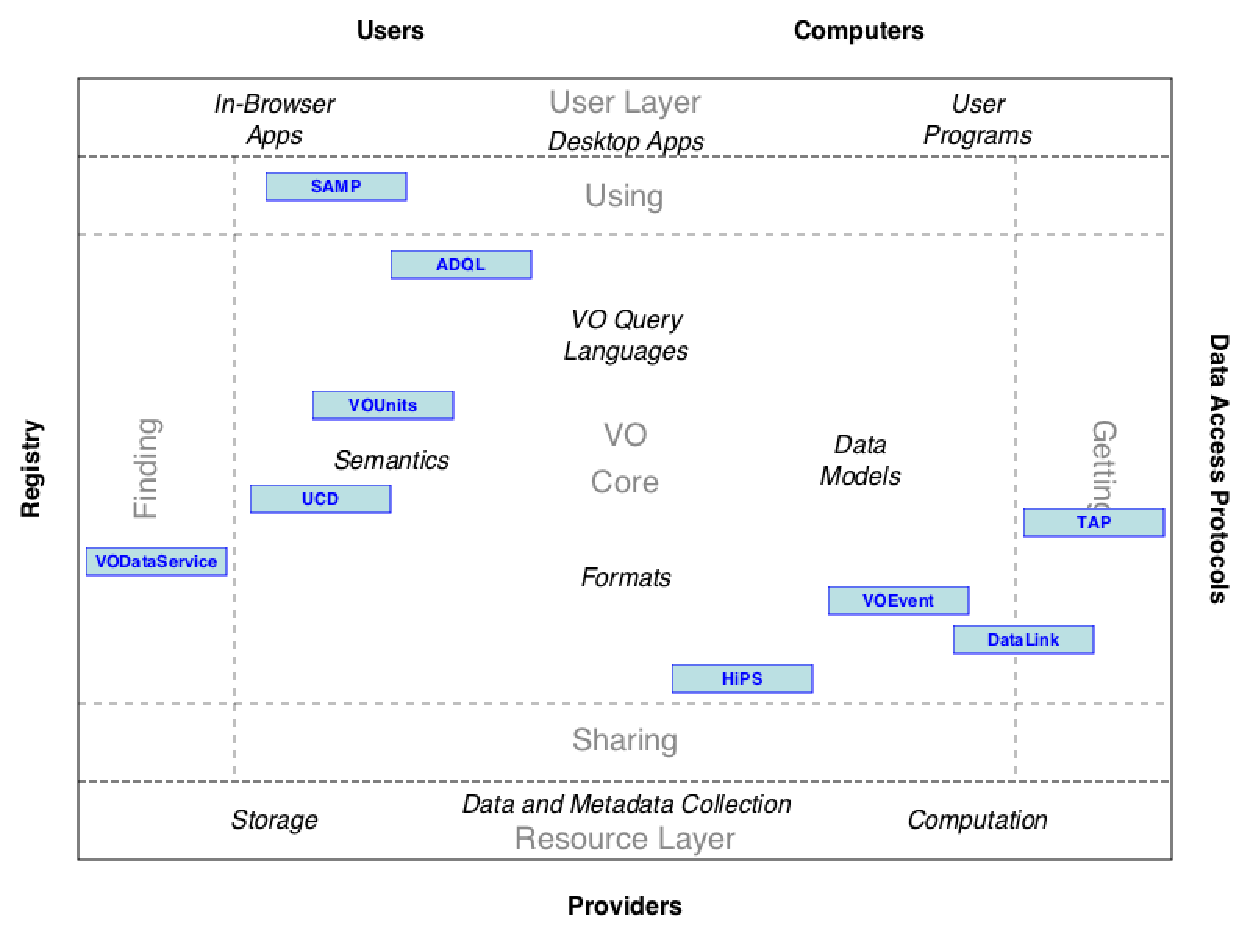
\includegraphics[width=0.9\textwidth]{role_diagram.pdf}
\caption{Architecture diagram for this document}
\label{fig:archdiag}
\end{figure}

Figure~\ref{fig:archdiag} shows how EPN-TAP fits into Virtual
Observatory architecture.  EPN-TAP's main connections to other VO
standards are:

\begin{bigdescription}
\item[ADQL \citep{2008ivoa.spec.1030O}] ADQL is the preferred language to
query EPN-TAP in.  The common language is a prerequisite for global
discovery within all EPN-TAP services.
\item[TAP \citep{2019ivoa.spec.0927D}] TAP is used to transport queries,
table metadata, and the results of queries.  The re-use of TAP gives
EPN-TAP a wide range of client and server implementations.
\item[VODataService \citep{2010ivoa.spec.1202P}] VODataService tableSets
are used to discover EPN-TAP services in VO Registries.
\item[UCDs \citep{2021ivoa.spec.0616C}] UCDs associated to EPN-TAP
parameters provide context when manipulating EPNCore tables and result
VOTables. They also describe the physical quantities distributed in
services via the measurement\_type parameter, making searches by physical
quantity possible.
\item[DALI \citep{2017ivoa.spec.0517D}] DALI lays out several basic
conventions, including the serialization of data types like timestamps
and geometries.
\end{bigdescription}

\section{The EPNcore metadata keyword dictionary}

% GENERATED: python3 parse_source.py columndescription
% To ignore the following section,
% add 'Mandatory parameters' to IGNORED_SECTIONS
\subsection{Mandatory parameters}

\subsubsection{Granule references}

These 3 keywords must always be informed. If granule grouping is not
relevant, use a single value for granule\_gid (and obs\_id can be
identical to granule\_uid).

\paragraph{granule\_uid}

Identifier for this row. This parameter is a primary key in epn\_core
tables, i.e., no two different rows may share the same granule\_uid.

There can be only one file associated to a granule (plus possibly a
thumbnail for quick-look purpose in a search interface).

\paragraph{obs\_id}

Associates granules derived from the same data (e.g.\ various
representations / processing levels). May be the ID of the original
observation.

\paragraph{granule\_gid}

Associates granules of same type (e.g.\ same map projection, or geometry
data products) --- think of it as a simple and convenient way to group or
differentiate types of data.

When several files relate to the same data, this parameter helps
distinguishing them: this will allow the user to select the type of data
of interest.  For instance, a service may provide links to calibrated images,
plus raw data and ancillary information for every observation; these
will share the same obs\_id, but will have different granule\_gid.

\subsubsection{Data Description}

\paragraph{dataproduct\_type}

The dataproduct\_type parameter describes the high level scientific
organization of the data product linked by the access\_url parameter,
or directly included in the table (in which case the value is `ci'
for catalogue\_item). EPNCore currently defines several types listed
below. The data provider must select the type most adapted to his
data. In complex situations (e.g., when a file contains several data
products), several types can be used to describe the same granule by
using a hash-separated-list — although using several granules to
describe the file content may be a better solution.

In EPN-TAP these types are identified by a 2-characters ID, so that
multivalued queries are unambiguous. Possible IDs are listed below with
their meaning:

\begin{itemize}

\item \textbf{im }(= image): scalar field with two spatial axes, or
association of several such fields, e.g., images with multiple color
planes, from multichannel or filter cameras. Preview images (e.g.\ map
with axis and caption) also belong here. Conversely, vectorial 2D fields
are described as spatial\_vector (see below).

\item \textbf{ma }(= map): scalar field / rasters with two spatial axes
covering a large area and projected either on the sky or on a planetary
body, associated to spatial\_coordinate\_description and map\_projection
parameters (with a short enumerated list of possible values); each pixel
is associated to 2D coordinates (e.g., fits with WCS). This is mostly
intended to identify radiometrically calibrated and orthorectified
images with complete coverage that can be used as reference basemaps,
but this also includes HiPS.

\item \textbf{sp }(= spectrum): measurements organized primarily along a
spectral axis, e.g., radiance spectra. This includes spectral aggregates
(series of related spectral segments with non-connected spectral ranges,
e.g., from several channels of the same instrument, various orders from
an échelle spectrometer, composite spectra, SED, etc).

\item \textbf{ds }(= dynamic\_spectrum): consecutive spectral measurements
through time, organized primarily as a time series. This typically
implies successive spectra of the same target / field of view.

\item \textbf{sc }(= spectral\_cube): sets of consecutive
spectral measurements with 1 or 2D spatial coverage, e.g., imaging
spectroscopy. The choice between image and spectral\_cube is dictated by
the characteristics of the instrument (which dimension is most resolved
and which dimensions are acquired simultaneously). The choice between
dynamic\_spectrum and spectral\_cube is related to the uniformity of
the field of view and by practices in the science field.

\item \textbf{pr }(= profile): scalar or vectorial measurements along
1 spatial dimension, e.g., atmospheric profiles, atmospheric paths,
sub-surface profiles, traverses…

\item \textbf{pf }(= photometric\_function): scalar or vectorial
measurements along 1 angular dimension, e.g., phase or polarization
curves, phase functions, emission-phase function sequences… Does not
handle variations along several angular axes. This is typically associated
to variations in illumination angle parameters.

\item \textbf{vo }(= volume): measurements with 3 spatial dimensions,
e.g., internal or atmospheric structures, including shells/shape models
(3D surfaces).

\item \textbf{mo }(= movie): sets of chronological 2D spatial measurements
(consecutive images)

\item \textbf{cu }(= cube): multidimensional data with 3 or more axes,
e.g., all that is not described by other 3D data types such as spectral
cube or volume. This is intended to accommodate unusual data with multiple
dimensions. This can be used for 3D ancillary data associated to spectral
cubes, e.g., providing the coordinates or illumination angles for
each spectrum.

\item \textbf{ts }(= time\_series): measurements organized primarily
as a function of time (with exception of dynamical spectra and movies,
i.e.\ usually a scalar quantity). Typical examples of time series include
space-borne dust detector measurements, daily or seasonal curves measured
at a given location (e.g.\ a lander), and light curves.

\item \textbf{ca }(= catalogue): applies to a granule providing a
catalogue of object parameters, a list of features, a table of granules
in another TAP service, a list of events, a list of spectral lines\dots The
result metadata table of a service query can also be considered as a
catalogue. Catalogues can be provided as VOTable (possibly containing
multiple tables, although this is not supported by SAMP). It is good
practice to describe the type of data included in the catalogue using
a hash-separated-list (e.g., a table of spectra should be described by
ca\#sp, so that it will respond to a query for spectra).

\item \textbf{ci }(= catalogue\_item): applies when the service itself
provides a catalogue with entries described as individual granules, in
particular when there is no associated file (e.g., a list of asteroid
properties or spectral lines). Catalogue\_item can be limited to scalar
quantities (including strings), and possibly to a single element. This
organization allows the user to search inside the catalogue from
the TAP query interface. In practice, Spice kernels are identified as
catalogue\_items because they are usually associated to a set of scalar
parameters.

\item \textbf{sv} (= spatial\_vector): vector information associated
to localization, such as a spatial footprints, a GIS-related element,
etc —  e.g.\ a kml or geojson file (STC-S strings are provided though
the s\_region parameter, though). This includes maps of vectors, e.g.,
wind maps.

\item \textbf{ev} (= event): introduces individual VOevents
formatted according to IVOA standard (or possibly events with other
formatting). Characteristics are provided via the event\_* parameters.

\end{itemize}

\textbf{\\}
\emph{Example TAP queries}:

\begin{verbatim}
SELECT * FROM pipo.epn_core
WHERE dataproduct_type LIKE '%im%'
\end{verbatim}

or

\begin{verbatim}
SELECT * FROM pipo.epn_core
WHERE ivo_hashlist_has(dataproduct_type, 'im') = 1
\end{verbatim}

will return only image data (the second syntax handles lists of values).

\paragraph{measurement\_type}

The measurement\_type parameter defines the physical quantities
contained in the data, using UCDs. It relates to the reported quantity,
not to the type of experiment. Therefore, only UCDs related to physical
quantities can be used; e.g., phys.absorption;em.opt.I is eligible,
while stellar\_occultation is not. This is used in particular to provide
indications to visualization/processing tools.

The ``UCD1+'' list from IVOA must be used as a
reference. New UCDs relevant for Solar System studies
are regularly discussed, therefore recent extensions
of this list must be also considered (i.e., at time of writing:
\url{http://www.ivoa.net/documents/UCD1+/20180527/index.html},
and Requests For Modifications).

Whenever several quantities are comprised in the data, the
measurement\_type parameter must describe all these quantities, using
multiple UCDs in a hash-separated-list.

\textbf{\\}
\emph{Example}:

\begin{itemize}
\item For images in general (i.e., actual measurements with a camera),
the relevant UCD is obs.image (or obs.image;stat.uncalib if not
calibrated).

\item For spectra: phot.radiance describes radiance, phys.reflectance
stands for reflectance factor (= I/F), and phot.flux.density for a
\emph{flux} vector (irradiance). The associated spectral vector is
described by UCDs em.wl, em.freq or em.energy, and the related error
has the form stat.error;phys.reflectance (for I/F).

\item Quantities derived from modeling/simulation are described by the
regular UCD with ``;meta.modelled'' appended.
\end{itemize}

\paragraph{processing\_level}

The processing\_level parameter is intended to provide the user with
a quick evaluation of data readiness level. When the original data collection
uses a specific encoding of processing levels, this one should be used
to meet the expectations of historical users; e.g., a service deriving
from a telescopic archive will preferably use the processing levels
from this archive. When no practice exists for a data collection, EPN-TAP uses
a simplified version of CODMAC / PDS3 levels as described below.

Several classifications are in use in different contexts, as summarized
in the table below.  EPNCore uses the CODMAC / PDS3 levels but removes
the intermediate calibration levels; this is equivalent to using the
simplified PDS4 levels and maintaining a separate level for ancillary
data. ``Partially calibrated'' data collections are in general considered as not
calibrated, but this evaluation is up to the data provider, depending on
context. ``Ancillary'' data include all extra information documenting
the measurements, in particular coordinates or geometry files. Several
processing levels can be included in the same service (in particular
calibrated and ancillary data, but also raw data). When mixed in the
same file, several values may be provided as a hash-separated-list.

Most EPN\_TAP data services are expected to include Calibrated or
Derived data.

\begingroup\small\begin{inlinetable}
\begin{tabular}{lllllp{2cm}lp{0.35\textwidth}}
\sptablerule
\vbox{\vskip 2pt\hbox{EPN-}\vskip 3pt\hbox{TAP2}}
&CODMAC&PSA&NASA&PDS3&PDS4&ObsTAP&Description\\
\sptablerule

1 &1 (raw)&(0?)&&UDR&Telemetry&0
  &Unprocessed Data Record (low-level encoding,
   e.g.\ telemetry from a spacecraft instrument.
   Normally available only to the original team)\\
2 &2 (edited)&1&0&EDR&Raw&1
  &Experiment Data Record (often referred to as ``raw data'':
   decommutated, but still affected by instrumental effects)\\
2?&\_&&&\_&Partially calibrated&
  &Processed beyond the raw stage,
   but have not yet reached calibrated status (PDS4)\\
3 &3 (calibrated)&2&1A&RDR&Calibrated&2
  &Reduced Data Record (``calibrated'' in physical units, no resampling)\\
5 (yes, 5)&4 (resampled)&&1B&REFDR&Derived&3
  &Reformatted Data Record
   (mosaics or composite of several observing sessions,
   involving some level of data fusion)\\
5 &5 (derived)&3&2-5&DDR&Derived&4
  &Derived Data Record
   (result of data analysis, directly usable by other communities
   with no further processing)\\
6&6 (ancillary)&&&ANCDR&Derived&
  &Ancillary Data Record
   (extra data specifically supporting a data set,
   such as coordinates, geometry… but also dark currents, flat fields…) \\
\end{tabular}
\end{inlinetable}\endgroup

Notes:

\begin{itemize}
\item This table is a compilation of information from
      PSA, PDS4, and ObsCore documents
\item The PDS3 column corresponds to the PDS3/PSA PRODUCT\_TYPE keyword
\item Descriptions are extracted from PSA and PDS4 documentations,
      with comments.
\end{itemize}

\subsubsection{Target description}

\paragraph{target\_name}

The target\_name parameter identifies a target by name or ID. The
target may be any Solar System body, exoplanet, planetary sample, or
meteorite, plus in some cases astronomical objects or spacecraft. Any
other feature (craters, regions, atmospheric layers\dots) must be named
using the optional feature\_name parameter (see 4.3.3). This parameter
can be multivalued only to describe several targets related to a granule
(e.g.\ with events). Alternative names of the same target must not be
listed here, but may be provided through the optional alt\_target\_name
parameter. In some rare cases no target name can be defined, so this
parameter can remain empty.

The best practice is to use the official designation of the target as
defined by IAU. This parameter is case sensitive (mixing lower/upper
cases) and all values must use the standard spelling and case; unusual
characters (such as intermediate spaces) are allowed, except quotes
and hashes (preferably changed to \_).
Data providers must be aware that services
which do not use the IAU designations might not be accessible by the
clients. Conversely, users must be aware that some services containing
data of interest might not be visible if they do not use the recommended
IAU nomenclature for planetary bodies. The quaero name resolver
(\url{https://ssp.imcce.fr/webservices/ssodnet/api/quaero/})
from IMCCE may help data providers (as well as users) to handle multiple
denominations; it is available from the VESPA portal to support queries.

Concerning celestial objects (at fixed position, i.e., stars,
galaxies…) the name should be identifiable through
Simbad\footnote{\url{http://simbad.u-strasbg.fr/simbad/}}.

Other best practices are listed below:

\begin{itemize}
\item The Exoplanet Encyclopedia provides a nearly
complete list of currently known extrasolar planets:
\url{http://exoplanet.eu/index.php}
(also available as an EPN-TAP service)

\item Meteorite catalogues can be found here:\\
\url{http://www.nhm.ac.uk/research-curation/research/projects/metcat/search/indexsing.dsml}
\\and
\url{http://www.lpi.usra.edu/meteor/index.php}.

\item The catalog of lunar samples is available here:
\url{http://www.lpi.usra.edu/lunar/samples/}

\item Other planetary samples are listed in topical web sites,
e.g.\ samples from the Stardust mission are described here:\\
\url{http://curator.jsc.nasa.gov/stardust/catalog/}

\item Consortia such as the IGSN\footnote{\url{https://www.igsn.org}}
issue IDs for samples

\item Asteroids: Usage is to use preferably name (if it exists) or
principal designation (the number is not used here, it can be included
in alt\_target\_name)

\item Meteors: the IAU Meteor Data Center assigns IDs to meteors and
meteor showers

\item Calibration targets: values can relate to existing names in a
given archive (e.g., the PSA contains values such as bias, checkout,
dark, flatfield, internal source…)
\end{itemize}

\textbf{\\}
\emph{Example TAP queries}:

\begin{verbatim}
SELECT * FROM pipo.epn_core
WHERE (target_name LIKE '%Ceres%' OR target_name LIKE '%Vesta%')
AND (target_class LIKE '%dwarf_planet%' OR target_class LIKE '%asteroid%')
\end{verbatim}

or

\begin{verbatim}
SELECT * FROM pipo.epn_core
WHERE (target_name LIKE '%Ceres%' OR target_name LIKE '%Vesta%')
AND (ivo_hashlist_has(target_class, 'dwarf_planet') = 1 OR
     ivo_hashlist_has(target_class, 'asteroid') = 1)
\end{verbatim}

Will return data only from 1 Ceres or 4 Vesta.

The LIKE operator is used here to handle cases when 1) the name includes a
number, either `1 Ceres' or `(1) Ceres', which (although not recommended)
may occur in some services, 2) the special case of dwarf planets, which
may be tagged as asteroids, or as `dwarf\_planet\#asteroid' (recommended,
see below).

The usage of LIKE cannot be generalized to all target\_class values,
because of  `planet' which also responds to `dwarf\_planet'.
The ivo\_hashlist\_has function smoothly handles all values
of target\_class.

\textbf{\\}
\emph{Example}:

1P is the official IAU designation for comet Halley

\paragraph{target\_class}

The target\_class parameter identifies the type of the target. Solar
System bodies are defined without ambiguity by the couple target\_class
and target\_name. In other cases, targets may have no proper name
(i.e., samples), but the target\_class parameter must be informed in
all cases. The possible values for target\_class are:

\begin{itemize}
\item asteroid
\item dwarf\_planet
\item planet
\item satellite
\item comet
\item exoplanet
\item interplanetary\_medium
\item sample
\item sky
\item spacecraft
\item spacejunk
\item star
\item calibration
\end{itemize}

Usage:

\begin{itemize}

\item Any target has a unique target class.

\item It is however good practice to use a hash-separated-list to
associate dwarf\_planet\#asteroid, so as to remove any ambiguity
(e.g., to help support older catalogues).

\item If several target\_name values are provided for a granule, 
several target\_class may be present as hash-separated values.

\item ``interplanetary\_medium'' refers in particular to interplanetary
dust observed in context (not to samples), or to simulations
(e.g., of primordial nebula).
Details can be provided through target\_region.

\item ``sample'' refers to lunar or planetary samples, to meteorites,
but also to terrestrial samples, e.g., in laboratory studies.

\item ``satellite'' stands for natural satellites only --- artificial
satellites are handled though spacecraft or spacejunk.

\item ``star'' is used typically for calibration targets, and for the Sun.

\item ``sky'' should be used for all other celestial bodies,
usually referred to by their sky coordinates.
It also includes the Interstellar Medium.

\item ``calibration'' is used for observations only related to instrument
or signal calibration, including dark current, flat field, reference
sample (in lab), etc (use of ``calibration'' with planetary bodies is
left to data providers).

\item planetary rings are not considered a target class, but appear in
target\_region with their planet indicated in target\_name.

\end{itemize}

\emph{Comment}:

All ``Types'' of objects used by the quaero resolver are included
in the EPNCore list: ``asteroid'', ``spacecraft'', ``comet'',
``exoplanet'', ``spacejunk'', ``satellite'', ``planet'', ``dwarf planet'',
``star''.\\Additional EPNCore classes are: ``interplanetary\_medium'',
``sample'', ``sky'', ``calibration''.


\subsubsection{Axes}

EPN-TAP describes the data coverage along 8 main axes:
time, spectral, spatial (3 coordinates), and viewing geometry (3 angles).

Coverages along the time/space/spectral axes are described with a range
and a resolution and/or sampling step.

Each quantity is a set of 2 parameters providing min and max values. They
must both be present with the same value when min = max. Additional single
parameters provide extra information: spatial\_frame\_type, s\_region,
and the optional shape parameter.

\paragraph{time (min/max)}

The time\_min and time\_max parameters provide the date and time of
acquisition in the observer frame.

The time parameters are always provided in UTC and formatted in Julian
Days (expressed in double precision). EPNCore uses standard JD to avoid
ambiguity with time origin (as opposed to ObsCore which uses Modified
JD). The use of double precision floats insures an accuracy on the order
of 1 ms, which is considered sufficient for search purposes (the initial
accuracy is preserved in the data itself). A client front-end may expose
times formatted in a more convenient way for human users.

\textbf{\\}
\emph{Example TAP queries}:

\begin{itemize}
\item Search data described by a time range:
\end{itemize}

\begin{verbatim}
select * from pipo.epn_core where time_min > '2455197.5' and time_max < '2455927.5'
\end{verbatim}

\begin{itemize}
\item Search data described by a start time parameter
\end{itemize}

\begin{verbatim}
select * from pipo.epn_core where time_min between '2455197.5' and '2455927.5'
\end{verbatim}

Time range is by default provided in the observer frame (i.e., at the
observer location at that moment), which is almost always the native time
in the data. For instance, space-borne observations are usually documented
with spacecraft on-board time, which is expected here (provided as JD,
not as on-board clock timing). For other cases, the location where time
is measured must be provided though the time\_refposition parameter.

To support space-borne vs ground-based campaigns, multiple spacecraft
observations, or survey of periodic events, measurement times need to be
corrected for light path. Whenever comparisons are potentially involved,
the use of the target\_time\_min and target\_time\_max parameters is
recommended in addition to time\_min and time\_max to make this kind of
comparison simpler.

Non-compulsory parameters may be used to accommodate additional,
specially formatted time scales such as native on-board time for space
borne observations. The information of the time\_min and time\_max
parameters is however highly recommended for all observations,
as it is used by default to search data collections.

\paragraph{time\_sampling\_step (min/max)}

These parameters provide the sampling step in seconds for measurements
of dynamical phenomena, and for computations. This is the time between
2 successive measurements or data, which is mostly relevant when the
measurements are regularly spaced. This may also reflect an input
parameter, e.g., for simulations or ephemeris computations. This
parameter is intended to allow the user to search for time-resolved
observations of dynamic phenomena, but can also accommodate the
``repetition time'' for several types of instruments.

\paragraph{time\_exp (min/max)}

These parameters correspond to the integration time (or exposure
time) of measurements in seconds. They provide an estimate of the time
resolution for dynamical phenomena, as well as an indication of relative
S/N ratio inside a given data collection. This time is usually shorter than
the time\_sampling\_step if both are present. It provides the overall
integration time, i.e.\ individual exposure time $\times$ number of summed
frames when relevant.

\paragraph{spectral\_range (min/max)}

The spectral\_range parameters define the upper and lower bounds of the
spectral domain of the data. This quantity is conventionally expressed
on a frequency scale in Hertz, although the client front-end may propose
conversions to other units/scales. The spectral range and associated
parameters only apply to electromagnetic waves. See the optional
parameters particle\_spectral\_* for particle energy or mass detection.

Since this is the standard parameter to identify a spectral range, it
is recommended to fill it even for images obtained through a filter
(for instance, by giving the central wavelength $\pm$ FWHM/2, 
or even just the central wavelength as both minimum and maximum,
which may already be enough to make the granule findable). 
The SVO Filter Profile 
Service\footnote{\url{http://svo2.cab.inta-csic.es/theory/fps3/}}
provides responses for many instrument filters;
bandwidths can be retrieved easily with a python library:
\url{https://github.com/hover2pi/svo_filters}.

\textbf{\\}
\textbf{Conversions}

\begin{verbatim}
with c = 2.99792458E8 (m/s)
spectral_range_min  = c*E6 /spectral_range_max_micron
spectral_range_max  = c*E6 /spectral_range_min_micron
(notice the inversion)
\end{verbatim}

\paragraph{spectral\_sampling\_step (min/max)}

The spectral\_sampling\_step parameters provide the spectral separation
between the centers of two adjacent filters or channels. Similar to the
spectral\_range quantities, they are expressed on a frequency scale in Hz.

These parameters are most relevant for radio observations
(long wavelengths / low frequencies) with regular sampling.
They can also help distinguish between Nyqvist and sub-Nyqvist
sampling rates (together with resolution).

\textbf{\\}
\textbf{Conversions}

\begin{verbatim}
with c = 2.99792458E8 (m/s)
df = c*1E6 dlam / lam^2 (from wavelength, with lam and dlam in micron)
df = c*1E3 dlam / lam^2 (same if dlam provided in nm)
df = c/1E-2 du (from wavenumber u in cm-1)
\end{verbatim}

\paragraph{spectral\_resolution (min/max)}

The spectral\_resolution parameters provide the (dimensionless)
resolving power $\lambda/\Delta\lambda = \nu/\Delta\nu$.

These parameters are mostly intended to provide an order of magnitude,
e.g., to distinguish between Fourier spectrometers, grating spectrometers
or filter cameras, or between observations related to surfaces or
atmospheres. This is often most relevant for optical/infrared observations
(short wavelengths / high frequencies).

\textbf{\\}
\textbf{Conversion}

\begin{verbatim}
spectral_resolution_min  = abs( spectral_range_min_micron / max(DeltaLambda) )
spectral_resolution_max  = abs( spectral_range_max_micron / min(DeltaLambda) )
\end{verbatim}

\paragraph{c1 (min/max)}

\paragraph{c2 (min/max)}

\paragraph{c3 (min/max)}

These parameters provide up to three spatial coordinates of the measured
target. The coordinates depend on the spatial\_frame\_type parameter
defined below. All services must handle three spatial coordinates,
even if the third one is always set to NULL. Some coordinates are
measured along a circle and must handle 0-meridian crossing, therefore
min/max values are actually start/stop values defining the footprint. In
body-fixed coordinates, c1 is longitude and is always counted eastward;
c1min is therefore the westernmost longitude and c1max the easternmost
one; the opposite applies to Right Ascension on the sky. Note that the
c3 parameter is related to the observed area, relative to a reference
surface in most cases; the target distance (e.g., geocentric distance
for ground based observations, or spacecraft distance) is introduced by
the optional parameters  ``earth\_distance'' or ``target\_distance''.

\textbf{\\}
\emph{Example TAP queries}:

Requests on C1/C2 coordinates often involve comparisons between two
bounding boxes. Below are typical examples in body-fixed coordinates,
when poles are not included in the bounding box.
\begin{description}
\item[Increasing longitudes: data range intersects {[100, 200]}:]\mbox{}
\begin{verbatim}
SELECT * FROM vvex.epn_core
 WHERE ((c1min <= c1max AND c1min <= 200.0 AND c1max >= 100.0) OR
        (c1min > c1max AND (c1min <= 200.0 OR c1max >= 100.0)))
   AND c2max >= -20.0 AND c2min <= 20.0 AND spatial_frame_type = 'body'
\end{verbatim}

\item[0-crossing longitude range: data range intersects {[300, 20]}:]\mbox{}
\begin{verbatim}
SELECT * FROM vvex.epn_core
 WHERE (c1min <= 20.0 OR c1max >= 300.0 OR c1min > c1max)
   AND c2max >= -20.0 AND c2min <= 20.0 AND spatial_frame_type = 'body'
\end{verbatim}

\item[Increasing longitudes: data range is included in {[100, 200]}:]\mbox{}
\begin{verbatim}
SELECT * FROM vvex.epn_core
 WHERE c1min >= 100.0 AND c1max <= 200.0 AND c1min <= c1max
   AND c2max <= 20.0 AND c2min >= -20.0 AND spatial_frame_type = 'body'
\end{verbatim}

\item[0-crossing longitude range: data range is included in {[300, 20]}:]\mbox{}
\begin{verbatim}
SELECT * FROM vvex.epn_core
 WHERE ((c1min >= 300.0 AND c1max <= 20.0) OR
        (c1min >= 300.0 AND c1max >= 300.0) OR
        (c1min <= 20.0 AND c1max <= 20.0))
   AND c2max <= 20.0 AND c2min >= -20.0 AND spatial_frame_type = 'body'
\end{verbatim}
\end{description}

In order to make uniform requests possible, spatial coordinates provided
in the EPNCore table must be standardized. However, they can be provided
in several systems types, as defined by the spatial\_frame\_type
parameter. The native coordinate system used in the EPNCore table can
be described by parameters spatial\_coordinate\_description and
spatial\_origin. This is intended to provide this information
prior to loading the data, especially when several coordinate
systems are available in the same service. Descriptions for EPN-TAP
are provided in a separate document (draft here: Planetary Coordinate
Systems\footnote{\url{https://voparis-wiki.obspm.fr/display/VES/Planetary+Coordinate+Systems}}).
Secondary coordinates can be introduced using additional parameters,
e.g., c1 and c2 ranges identify the visible region of a planetary
disk, while extra RA / Dec parameters provide location on the
sky at this moment, and subobserver\_longitude\_min/max and
subobserver\_latitude\_min/max provide the coordinates of the disk center.

\paragraph{c1\_resol (min/max)}

\paragraph{c2\_resol (min/max)}

\paragraph{c3\_resol (min/max)}

These parameters provide a simple estimate of the resolution in the same
frame/units as c1/c2/c3. For instance, if spatial\_frame\_type =
`celestial', it can accommodate the FWHM of the PSF on the sky (in
degrees). The client front-end may propose more appropriate units to the
user, depending on context (e.g., angular resolution in mas, distance
in m\dots).

\paragraph{spatial\_frame\_type}

Provides the ``flavor'' of the coordinate system, which defines the nature
of the spatial coordinates (c1,c2,c3) in the EPNCore table and queries,
and the way they are defined. A value is always required (use ``none''
if not applicable, although ``body'' is found in older services and may
be OK). This may be different from the coordinate system associated to /
included in the data themselves. The reference frame itself is defined by
the spatial\_coordinate\_description parameter, and the frame center can
be specified using the spatial\_origin parameter in case of ambiguity.
The possible types are described below:

\begin{itemize}
\item \textbf{celestial}: 2D angles on the sky, i.e., right ascension
c1 and declination c2 plus possibly the heliocentric distance in c3 (in AU);
although this is a special case of a spherical frame, the order and
conventions are different. Right ascension is provided in degrees. ICRS
coordinates are assumed by default, but other frames may exist, e.g.\ HPC
(Helio-Projective Cartesian) is centered on the Sun; such frames are
identified from the spatial\_coordinate\_description parameter.
For ground-based observations, Earth distance may be provided in the
earth\_distance parameter (not in c3).

\item \textbf{body}: 2D angles in body-fixed frame: longitude c1 and
latitude c2 plus possibly altitude as c3. \\A planetocentric system with
eastward longitudes in the range (0,360)° is required for service
interoperability. Current IAU frame is assumed, in particular for
definition of the prime meridian. IAU 2009 planetocentric convention
applies, in particular eastward longitudes and a north pole located on
the north side of the invariant plane of the Solar System for planets
and satellites.  \\Parameter c3 is measured above the reference
ellipsoid, and can be <0 for interiors. Two other parameters are
available to provide other vertical scales if needed (radial\_distance
and altitude\_fromshape). \\Planetocentric rotating frames are defined
as spherical (rather than body).

\item \textbf{cartesian:} (x,y,z) as (c1,c2,c3).
This includes spatial coordinates given in km.

\item \textbf{spherical:} (r, theta, phi) as (c1,c2,c3), as
defined in ISO standard 80000-2:2009; r = radius; theta = zenith
angle/colatitude/inclination; phi = azimuth (E longitude). Angles are
provided in degrees. When related to the sky or tied to a solid body,
``celestial'' (with RA/Dec) or ``body'' (with E longitude/latitude)
frames must be used instead.

\item \textbf{cylindrical:} (r, theta, z) as (c1,c2,c3); r = radius in
km; theta = azimuth; z = height in km. The angle is provided in degrees.

\item \textbf{none:} to be used when no spatial frame is defined for
the data. This value is intended to prevent useless searches when space
coordinates are not defined (a non-zero value is required by the mixin
in DaCHS).

\end{itemize}

This parameter, although related to the specific coordinate system in use,
is mostly intended to identify the nature of the coordinates provided in
the service table (e.g., angles versus distances). This parameter is
provided as a column of the EPNCore table to ensure it can be queried
through the basic TAP mechanism. Although it will in general remain
constant along the table for simple services, this parameter can vary from
granule to granule and a value must therefore be provided in any query
that includes spatial coordinates. Whenever additional coordinates are
provided, they must be stored in extra columns of the table. If several
different frames are mixed to provide the main coordinates, the use of
different granule\_gid may help clarify the situation. At any rate, easy
access to the data must be considered during the design of the service.

\paragraph{incidence (min/max)}

The incidence parameters define the upper and lower bounds of the
incidence angle range in the data (also known as Solar Zenith Angle).
This is always indicated in decimal degrees, and usually ranges from 0 to
90° (with 0° indicating the normal to the surface). Incidence and
emergence angles may be counted relative to the normal of the ellipsoid
model, or to the local normal (e.g., using a 3D shape model). In case
the two systems are included in the data, these keywords introduce the
values relative to the ellipsoid (local values may be provided through
non-compulsory parameters).

\paragraph{emergence (min/max)}

The emergence parameters define the upper and lower bounds of the
emergence, emission, or viewing angle range in the data. This is always
indicated in decimal degrees, and usually ranges from 0 to 90° (with
0° indicating the normal to the surface). Incidence and emergence angles
may be counted relative to the normal of the ellipsoid model, or to the
local normal (e.g., using a 3D shape model). In case the two systems
are included in the data, these keywords introduce the values relative
to the ellipsoid (local values may be provided through non-compulsory
parameters).

\paragraph{phase (min/max)}

The phase parameters define the upper and lower bounds of the phase
angle range in the data (i.e., $\textrm{scattering angle} - 180^\circ$, or 
$\textrm{light source}-\textrm{target-observer angle}$. 
It is always indicated in decimal degrees,
and may range from -180 to 180° (with 0° corresponding to opposition,
i.e., light source in the back of the observer). Negative values may
refer, e.g., to geometry before opposition, depending on context.
Phase ($\phi$), incidence $i$ and emergence $e$ are partly related:
\begin{displaymath}
  |i - e| < \phi < i + e
\end{displaymath}

If the azimuth angle $a$ is available instead of the phase angle,
the latter can be derived from knowledge of the three angles:
\begin{displaymath}
  \cos(\phi) = \cos(i) \cos(e) + \cos(a) \sin(i) \sin(e)
\end{displaymath}

\paragraph{s\_region}

This parameter introduces a footprint as a contour. The s\_region
parameter should be given for geolocalized data products in 2D, most
notably on the sky (using RA, Dec) or on planetary surfaces (using E
longitude, latitude) to communicate the geometry of a feature or an
observation's footprint. This is a single parameter with no min/max
declinations. Coordinates are provided in the same reference system as
c1/c2 parameters, clients must therefore inspect spatial\_frame\_type
before interpreting such contours. Any type of contour that works with
ADQL's geometry operators (CONTAINS, INTERSECTS...) is legal here.

The shape parameter introduces another type of footprint, with potential
extension to time coverage. When both are present, care must be taken
that they are consistent.

In the VOTable serialization the s\_region parameter is represented
as either an STC-S string value with xtype='adql:REGION' or a DALI
1.1-compliant numeric array value with xtype='point', 'circle' or
'polygon'.

\textbf{\\}
\emph{Implementation notes:}

Two syntaxes are possible:

1) The original ObsCore s\_region one (currently limited to polygons)
— a string with syntax: `\{(lon1,lat1), (lon2,lat2), … \}' (with
no quotes) where (lon1,lat1) = (10.d, 5d), character d included (it
stands for degrees). Pairs (lon1,lat1) must sample the contour in a
sequence provided in direct (counter-clockwise) sense as viewed from
the observer. Notice that the result of a TAP query is an STC-S string,
which has different format (as in ObsCore).

2) Modern DALI 1.1 geometries — a numeric array providing either a point
(`lon lat', with no quotes), a circle (`lon lat radius', with no quotes),
or a polygon (sequence of at least 3 `lon lat' pairs, with no quotes). For
polygons, pairs (lon lat) must sample the contour in a sequence provided
in direct (counter-clockwise) sense as viewed from the origin (when on
the sky) or from the observer (when on planets).

\subsubsection{Data origin}

\paragraph{instrument\_host\_name}

This parameter provides the name of the observatory, spacecraft, or
facility that performed the measurements. A hash-separated-list of host
names must be provided for integrated data sets. In the EPNCore table, the
acronym is preferred to the full name to avoid long strings and related
errors (both values can be provided in the list). An observatory list
is being developed in Europlanet-2024/VESPA and will be implemented in
a resolver by merging existing lists (draft here: Observatory Facility
Database\footnote{\url{https://voparis-wiki.obspm.fr/display/VES/Observatory+Facility+Database}}).

\textbf{\\}
Reference lists include:

\begin{itemize}
\item for ground-based observations, the list of IAU observatory
codes:\\
\url{http://www.minorplanetcenter.net/iau/lists/ObsCodesF.html}
\\However, this list is not intended to include all ground-based
observatories, and a complement still needs to be identified (including
e.g.\ radio-telescopes).

\item a reasonably complete list of radio-telescopes is available here:\\
\url{http://en.wikipedia.org/wiki/List_of_radio_telescopes}

\item the WiseRep list also
provides a  database of telescopes and instruments:\\
\url{https://wiserep.weizmann.ac.il/aux/telescopes}\\
\url{https://wiserep.weizmann.ac.il/aux/instruments}

\item Concerning space-borne data, the most complete list of
international planetary missions and orbital observatories is
found here (included in a complete list of space missions with ID):
\url{http://nssdc.gsfc.nasa.gov/nmc/}\\
Planetary missions are also listed here:
\url{http://nssdc.gsfc.nasa.gov/planetary/chronology.html}.

\item Alternatively, the PDS dictionary defines values
for many mission names:\\
\url{http://pds.nasa.gov/tools/dictionary.shtml}\\
Other mission names are supported by the SPICE system,
but only as ID codes:\\
\url{https://naif.jpl.nasa.gov/pub/naif/toolkit_docs/FORTRAN/req/naif_ids.html}
\end{itemize}

\paragraph{instrument\_name}

Identifies the instrument(s) that acquired the data.
A hash-separated-list of instruments must be provided
for integrated data products.
Service providers are invited to include multiple values
for instrument name, e.g., complete name and usual acronym.
This will allow queries on either
``VISIBLE AND INFRARED THERMAL IMAGING SPECTROMETER'' or ``VIRTIS''
to produce the same reply. For ground-based observations and lab
measurements, this is typically the name of the instrument in use (not
the telescope or facility). Non-compulsory parameters are available to
provide more information about sensors, instrument modes, etc.

\textbf{\\}
\emph{Example}:

\begin{verbatim}
VISIBLE AND INFRARED THERMAL IMAGING SPECTROMETER#VIRTIS
\end{verbatim}

A list of recommended values (to be implemented in
a resolver) is discussed here: Observatory Facility
Database\footnote{\url{https://voparis-wiki.obspm.fr/display/VES/Observatory+Facility+Database}}

The most complete ready-to-use list of international
planetary missions and orbital observatories is found here:
\url{http://nssdc.gsfc.nasa.gov/nmc/}

Instruments on board planetary missions in particular are listed here:\\
\url{http://nssdc.gsfc.nasa.gov/nmc/experimentSearch.do}

\subsubsection{Granule call-back info}

These parameters provide ancillary information for routine processing
after a query. These 4 keywords must always be informed.
Dates are provided in ISO 8601 format.

\paragraph{service\_title}

Provides an acronym for the service/table title and must be constant
throughout the service. This parameter may be used to refer to the service
providing the data (e.g.\ when handling multiservice results). When
designing the service, care must therefore be taken to use a title not
already ascribed to another EPN-TAP service. Special/unusual characters
must be avoided (including \#, ?, etc).

Other identifiers (ivoid…) may be used in a future version.

\paragraph{creation\_date}

Provides the date when the granule was introduced in the service.

\paragraph{modification\_date}

Provides the date when the granule was last updated.
This is intended to speed up mirroring between sites and to flag recalibrations.
When unknown or not relevant, the creation date is replicated here.

\paragraph{release\_date}

Provides the date when the granule becomes public.  This is
intended to support a proprietary period.
When unknown or not relevant, the creation date is replicated here.

% To ignore the following section, add 'Optional parameters' to IGNORED_SECTIONS
\subsection{Optional parameters}

\subsubsection{Data Access Reference}

If the data are not included in the table
(i.e., provided in separate files),
these 3 parameters must be present and informed. If alternative
formats are also provided, they must be described in other granules
with the same obs\_id and possibly different group ID. Whenever the
data consists of a few scalar fields, these parameters are best replaced
by parameters providing the data itself in the table.  This makes them
usable in query constraints (e.g.\ mass, in a table providing the masses of
Solar System bodies).

\paragraph{access\_url}

The data of interest are often stored in a file, not in the table itself.
In this very usual case, the access\_url parameter provides
a complete path to the data products on the network, so that they are
accessible for download by plotting or processing tools. All URLs in the
EPNCore table are case sensitive and must provide an actual and unique
link. The link may be a call to a web service (e.g., PlanetServer\_CRISM
service) or the output of a script (e.g., Titan atmospheric profiles
service); in both cases the link must include the adequate arguments. In
any case, this parameter must link to the actual data, not to a file of
metadata nor a document. Datalinks (which typically open a page with
either a list of links or an input interface for parameters) can be
used for this later purpose, and must be provided via the datalink\_url
parameter.

\paragraph{access\_format}

Access\_format provides the format of the data file linked through
the access\_url parameter. \\The data may be stored under native
format, and no format conversion is required to set up an EPN-TAP
service; this field can therefore include reference to unusual
formats. However, VO-ready formats are required to take advantage
of visualization and processing in VO tools. Consistently with
ObsCore, possible values are MIME-types written in lower case;
the most common ones are listed on this page: Data Formats and MIME
Types\footnote{\url{https://voparis-wiki.obspm.fr/display/VES/Data+Formats+and+MIME+Types}}.

\paragraph{access\_estsize}

The access\_estsize field provides an order of magnitude of the size (in
kilobytes) of the file available via the corresponding URL. It is intended
to provide an indication that can help to tune download functionalities
in an application, depending on data volume and transfer bit rate.

\textbf{\\}
\textbf{Other parameters may be used to describe the data files:}

\paragraph{thumbnail\_url}

The thumbnail\_url parameter contains the URL of a reduced version
of the data product used for quick-look purpose (e.g., a small jpeg
image, typically 200x200 pixels). This may be handy in the case of big
data files or unusual data formats, to facilitate data selection by the
user. EPN-TAP clients such as the VESPA portal use this thumbnail for
an on-line quick-look.  It therefore contributes significantly to a
service's accessibility. 
Preferred formats include jpeg and png, which are handled easily
in a web browser. Larger or more elaborate previews must be provided as
independent granules and identified via a granule\_gid different from
the data. All URLs in the EPNCore table are case sensitive and must
provide an actual link.

\paragraph{file\_name}

The file\_name parameter introduces the name of the \emph{data}
file, with extension but no path information. In many data services,
the file name encodes the most relevant metadata and may be a
very handy access mechanism for specialists. In services providing
sets of files in a complicated directory tree (e.g., related to
a spacecraft operation plan), the file\_name parameter is a handy
key to perform automatic operations such as mirroring, pipeline
processing, etc.  A web service is available to retrieve a file from
the file\_name parameter in any EPN-TAP service (File grabbing interface
(fgi)\footnote{\url{https://voparis-wiki.obspm.fr/pages/viewpage.action?pageId=17236008}}).
Its use is therefore always recommended when data are provided in separate
files, i.e., not included in the table.\\All file\_name values in the
EPNCore table are case sensitive and must reflect the filename of the
product provided through access\_url; for instance, if access\_url is
a link to a script converting an ascii file to VOTable, file\_name must
refer to the outcome of this script, in this case the VOTable.

\paragraph{access\_md5}

This parameter introduces a MD5 Hash for the file when available
(link to a real file), to be used as a checksum.

\paragraph{accref}

Although not an EPNCore parameter, this name is reserved for internal use.
It must not be used explicitly, as DaCHS uses it internally in some
situations (although it is not included in the answer to a TAP query):
it is used to introduce a URL with datalink (present in epncore2 mixin)
and is also generated automatically in the q.rd when using the localfile
mixin (when accessing data files located on the DaCHS server itself);
it may also be used to handle proprietary periods in DaCHS. \\

\paragraph{datalink\_url}

This parameter is used to provide extra accesses through a datalink/SODA
interface. It can either provide a table of hard links (dlmeta) or a
dialogue to setup input values on the fly and call a web service on
the data server (dlget). Links can be parameterized with input values
retrieved from the current granule at the time of ingestion; if several
EPN-TAP parameters need to be passed, they must be first concatenated
in an extra parameter in the table (often called \textbf{ds\_id}).

\subsubsection{Supplementary description}

\paragraph{bib\_reference}

The bib\_reference parameter introduces an individual bibliographic
reference at granule level. This provides the origin of the
data, e.g., if the resource is a compilation of data from various
origins. References are best provided as bibcode (as used e.g.\ by ADS),
as DOI, or as arXiv reference, although other formats are acceptable. A
generic regular expression for bibcode (from IPDA discussions) is:
[0-9]\{4\}[A-Za-z0-9$\backslash$\&$\backslash$.]\{5\}[A-Za-z0-9$\backslash$.]\{9\}[A-Z$\backslash$.]

See \url{http://adsabs.github.io/help/actions/bibcode}

\paragraph{publisher}

Specifies the publisher of the \emph{data service} (not necessarily at
the origin of the data). Currently a free format string.

\paragraph{internal\_reference}

The internal\_reference parameter can be used to identify granules
(or sets of granules) intimately related to the current one. e.g.,
in a service containing both observations and results of analysis of
observation sets, internal\_reference can be used to provide the set of
observations used to compute a result. This contains a hash-separated-list
of granule\_uid in the same service (which implies that those never
contain the \# character).\\This is specifically intended to provide
internal references in services which would otherwise need to be split
in several tables, and it must only be used as a last resort (clever
use of obs\_id and granule\_gid is usually more efficient).

\paragraph{external\_link}

The external\_link parameter can be used to provide extra information
that does not fit easily in the table, and is intended for human reading
only. This parameter must contain a single URL. This is typically an
extended discussion of a granule on a web site, which may include images,
tables, or other documents. For instance, the individual planet pages of
the Encyclopedia of exoplanets are linked with this parameter, as they
contain many links and sometimes web applets. Alternatively, the parameter
can provide a link to a web service related to this granule; for instance,
in the HRSC/MEx service (hrsc3nd) it displays a detailed view of the
image with zooming functions for quick examination at full resolution.

\paragraph{species}

The species parameter introduces the chemical species of interest in
simple data services. The formatting is very basic and simply uses the
standard formula in ascii, e.g., H2O for water, CO2 for carbon dioxide
or Fe for iron. This is one of the few query parameters provided in
case sensitive form, using the standard chemical notation. This format
can only accommodate atoms and simple molecular species, and does not
support isotopic variations.

An example application is related to atmospheric composition:
a table providing vertical profiles of gaseous species with altitude.
All columns are abundances and are described by the same measurement\_type
parameter. The use of the ``species'' parameter allows identifying the
various species and accessing the requested information. This of course
is restrained to simple cases.

If more elaborated compositional information must be included, the use of
parameter species\_inchikey is recommended. InChiKeys identify molecule,
including isotopes, but not the physical state or phase.

\paragraph{messenger}

This parameter is a generalization of waveband from VODataService
(used e.g.\ in ConeSearch and SSA). It provides a rough indication
of the spectral domain, e.g.\ when variable in a large archive. In
addition, values for messenger can describe particles other than
photons. Possible values are from the IVOA vocabulary (and case matters)
\url{http://www.ivoa.net/rdf/messenger}.

\paragraph{filter}

This parameter introduces the standard name of a filter used during
measurements. It is reserved for filters in imaging mode (no
grating/grism \#, etc). There is no predefined list, because of the large
variety of possible denominations, but the best practice is to use a short
and accurate ID. This VO service provides an extended list of references:
\url{http://svo2.cab.inta-csic.es/svo/theory/fps3/}

This is intended to document the results of a search, rather than
a search parameter. Therefore, it is recommended to also fill the
spectral\_range\_min/max parameters to describe filter imaging --- this
is the only way to make filter imaging easily searchable.

\paragraph{alt\_target\_name}

This parameter introduces alternative names of the target, especially
when they are more commonly used than the official IAU one (e.g., Halley vs 1P).

A frequent usage is to store a hash-separated-list of all alternative
names for small bodies to avoid ambiguities (e.g., for asteroids: name,
number, principal and provisional designations). Although this situation
never occurs for small bodies, care must be taken to replace possible \#
characters by \_ in target names (e.g., for samples).

\paragraph{feature\_name}

Introduces a supplementary name to provide more details
about the observed target. It is intended in particular to
accommodate a local name (crater, surface feature, region…)
whereas target\_name is reserved to identify the whole body
(Mars, Moon, Ceres…). Use of official features names defined by IAU
(\url{http://planetarynames.wr.usgs.gov/})
is preferred when relevant.

\paragraph{target\_region}

Specifies a \emph{type} of region on the target. This parameter
only introduces generic regions  (e.g., atmospheric layer, internal
structure…), not specific local names which must be handled using the
feature\_name parameter.

Values are best selected from the IVOA
rendition of the Unified Astronomy Thesaurus:
\url{http://www.ivoa.net/rdf/uat}

Older sources (some of them may be integrated in the UAT) include:

\begin{itemize}
\item IVOA thesaurus:
      \url{http://www.ivoa.net/rdf/Vocabularies/vocabularies-20091007/IVOAT/}
\item IAU thesaurus:
      \url{http://www.vocabularyserver.com/trex/en/}
\item Spase dictionary \url{http://www.spase-group.org/}
\end{itemize}

\textbf{\\}
\emph{Example}:

\emph{``atmosphere'', ``surface'', ``ionosphere''}\\
The same sources are used for the declaration file in the registry.

\paragraph{shape}

This parameter introduces a footprint as a MOC (healpix-based).
It is intended to support space/time coverages, most notably on the sky
(assuming RA, Dec coordinates) or on planetary surfaces (assuming
E longitude, latitude). This is a single parameter with no associated min/max
parameters. It must contain a MOC 2.0 ascii string (MOC or STMOC).
The result of the query must have xtype = ``MOC''
for proper handling in TAP.

The shape parameter may appear together with s\_region, which introduces
a simpler type of footprint (2D contour). Shape has precedence over
s\_region. When both are present, care must be taken that they are
consistent.

\subsubsection{Description of coordinate frame}

\paragraph{spatial\_coordinate\_description}

\paragraph{spatial\_origin}

These two parameters provide a description of the spatial frame in use,
depending on the spatial\_frame\_type parameter. Both parameters relate
to the coordinates provided in the EPNCore table, not necessarily to
those included in the data products.

Spatial\_coordinate\_description provides an acronym of the
Coordinate Reference System as discussed in Planetary Coordinate
Systems\footnote{\url{https://voparis-wiki.obspm.fr/display/VES/Planetary+Coordinate+Systems}}.
For body-fixed frames, IAU/SPICE/WMS strings such as IAU20xx:49900 are
eligible --- in this case, the final 00 which stands for planetocentric
E-handed is the only valid option (refers to EPN-TAP standard on c1/c2
coordinates). If absent the current IAU coordinate system is assumed,
depending on context.

Spatial\_origin may be used to identify frame center
in specific situations, using either target\_name
(referring to target center) or the IVOA vocabulary
(\url{http://www.ivoa.net/rdf/refposition}).
Other values may be used, e.g., to introduce specific geometries for
simulations.

\textbf{\\}
\emph{Examples}:

\begin{verbatim}
spatial_coordinate_description: ICRS, IAU_MARS, IAU2000:49900
spatial_origin: Geocenter, Mars, (spacecraft)
\end{verbatim}


Spatial\_coordinate\_description and an epoch derived from time\_min/max
can be used to feed the COOSYS element of VOTable 1.4 when its value
is constant throughout the table (notice that most EPN-TAP coordinate
frames are not standard values in this vocabulary at the time of writing):

\begin{verbatim}
<COOSYS ID="system" epoch="<epoch>" system="<spatial_coordinate_description>"/>
\end{verbatim}

\paragraph{time\_refposition}

Indicates where the time is measured, which can be a planet or a
spacecraft — this does not handle time zones on Earth. This knowledge
is required to cross-correlate event-based observations, in particular
to indicate light-path differences. It applies to the time\_min and
time\_max parameters (while target\_time\_min/max always refer to the
target in the FoV). If this parameter is not informed, time is expected
to be provided in the observer frame (related to instrument\_host\_name),
which is not necessarily fixed in the Solar System.

Values for time\_refposition may specify a target name (referring
to target center) or spacecraft name, or use the IVOA vocabulary
(\url{http://www.ivoa.net/rdf/refposition})
including future versions of the hierarchy proposed at
\url{https://wiki.ivoa.net/internal/IVOA/InterOpMay2019TDIG/topocenter.pdf}.

\textbf{\\}
\emph{Example}:

\begin{verbatim}
Geocenter, (solar system bodies), (spacecraft)
\end{verbatim}

\paragraph{time\_scale}

Provides the time scale applying to time\_min and time\_max parameters.
UTC is assumed when no value is provided, since this
is the expected value in most observational data services.
Some services (in particular computational ones) may need to specify
different time scales by using other using standard acronyms
— values are preferably taken from the IVOA vocabulary:
\url{http://www.ivoa.net/rdf/timescale}

Both time\_scale and time\_refposition can be used to feed the TIMESYS
element of VOTable 1.4 when their values are constant throughout the
table (this is best avoided otherwise, e.g., when grouping coordinated
observations from various locations in the Solar System):

\begin{verbatim}
<TIMESYS ID="time_frame" refposition="<time_refposition>"
         timeorigin="JD-origin" timescale="<time_scale>"/>
\end{verbatim}

\subsubsection{Target configuration and observing geometry}

The next pairs of parameters provide additional location in time and
space, and require min/max values. They are independent and can appear
separately:

\paragraph{solar\_longitude (min/max)}

Solar longitude (a.k.a. heliocentric longitude, or ecliptic longitude of
the Sun, traditionally noted Ls) is the Sun-Planet vector angle counted
from the planet position at N hemisphere spring equinox. It provides a
measurement of season.

Ls = 90° corresponds to the northern summer solstice, Ls = 180°
to the northern autumn equinox, and Ls = 90° to the northern winter
solstice. Although it is most usually applied to Mars and Titan (using
Saturn's Ls), this notion can be enlarged to any planetary body without
ambiguity.

This should not be confused with the true anomaly of the body (which
is the same angle counted from the perihelion position), nor with the
longitude of the subsolar point (see below).

\paragraph{local\_time (min/max)}

Provide the local time at the observed area. These parameters are
provided in unit of target rotation divided by 24 and are measured from
local midnight, i.e., in decimal (local) hours (range from 0 to 24,
must increase with time at a given location).

\paragraph{target\_distance (min/max)}

The target\_distance parameters introduce the distance of the observer
to the observed area (in km) along the line of sight. This is mostly
intended for space borne data, where it provides the spacecraft-target
distance in km. For ground-based observations the earth\_distance\_min/max
parameters should be used instead (in AU).

\paragraph{target\_time (min/max)}

The target\_time parameters introduce the time measured in UTC scale
at the target. This is intended to directly correlate simultaneous
observations such as ground-based support and space-borne observations,
or multi-spacecraft campaigns. Values in ISO 8601 format.

\paragraph{earth\_distance (min/max)}

\paragraph{sun\_distance (min/max)}

These two parameters provide the corresponding distance of Earth or Sun
to the target at the time of observation (in AU). When the target is the
Sun or Earth, use the target\_distance\_min/max parameters to provide
the distance to the observer.

\paragraph{subobserver\_longitude (min/max)}

\paragraph{subobserver\_latitude (min/max)}

Provide coordinates of sub-observer point, in particular sub-Earth
point (disk center) or central meridian for ground-based observations
(this is different from the FoV location which is provided in c1/c2
parameters). The min/max pair is required to support long exposures
related to time series, especially on giant planets to test target
attitude.

\paragraph{subsolar\_longitude (min/max)}

\paragraph{subsolar\_latitude (min/max)}

Provide coordinates of sub-solar point, especially for disk images.
The min/max pair is required to support long exposures
related to time series.

\paragraph{ra, dec}

Sky coordinates of the target can be provided in addition to standard
coordinates, in which case they must be stored in these parameters.
This may for instance document the location of a planet
in a celestial image,
while the main coordinates c1/c2 are used to provide the observed area as
longitude and latitude. ICRS coordinate system is assumed; right ascension
is provided in degrees (similar to ObsCore). RA and DEC parameters are
interpreted correctly by most VO tools, therefore no min/max variations
are allowed to maintain compatibility with existing software.

\subsubsection{Vertical scales on planets}

In body-fixed frame, parameters c3min/max, if present, introduce a
vertical range counted from a reference surface, typically the reference
ellipsoid for the current target. \\

Two other parameter pairs can be used provide different vertical
scales, and must be considered for atmosphere-related services when
available/relevant:

\paragraph{radial\_distance (min/max)}

Distance of observed area (at c1/c2) from body center, measured in km.
Not to be confused with target\_distance
(which provides the distance from observer to observed area).

\paragraph{altitude\_fromshape (min/max)}

Altitude of observed area (at c1/c2) above local surface, measured in km.
The local surface is provided by a DTM or a shape model.
This parameter typically provides the height in the atmosphere.

Parameter c3 can be used to select services/data in a given altitude
range above the ellipsoid, while radial\_distance and altitude\_fromshape
provide other convenient vertical scales to compare observations from
various origins. This use of c3min/max also applies to planetary interiors
(c3 is then <0) and measurements at high altitude/distance.

% To ignore the following section, add 'Extensions' to IGNORED_SECTIONS
\subsection{Extensions}

\subsubsection{Particle spectroscopy extension}

These parameters are related to the spectral distribution of particles
only -- for electro-magnetic waves, the spectral\_* parameters apply.

When used, these parameters define an extra axis and must all be present.
This set defines an additional axis for particle energy,
all with min/max values.

\paragraph{particle\_spectral\_type}

The particle\_spectral\_type parameter specifies the type of axis in use:
either `energy' (provided in eV), `mass' (in amu), or `mass/charge'
(in amu/qe).

\paragraph{particle\_spectral\_range (min/max)}

The particle\_spectral\_range parameters define the upper and
lower bounds of the spectral domain for particles. Depending on the
particle\_spectral\_type parameter, this quantity is expressed on an
energy, mass, or mass/charge scale, with respective units eV, amu,
or amu/qe.

\paragraph{particle\_spectral\_sampling\_step (min/max)}

The particle\_spectral\_sampling\_step parameters provide the
spectral separation between measurements, in the same scale and unit as
particle\_spectral\_range.\\
This parameter is mostly intended to provide an order of magnitude.

\paragraph{particle\_spectral\_resolution (min/max)}

The particle\_spectral\_resolution parameters correspond to the actual
resolution of the measurements, and are provided in the same scale and
unit as particle\_spectral\_range. \\
This parameter is mostly intended to provide an order of magnitude.

\subsubsection{Solar System Objects extension}

Service providing descriptions of solar system objects contain
no observations (only inferred properties).\\
In this case, the target\_distance\_min/max parameters
can provide distances from the frame origin (typically heliocentric),
in km for consistency --- TBC, not favorite

\paragraph{mean\_radius, equatorial\_radius, polar\_radius}

These parameters are used to provide solar system object sizes (in km)

\paragraph{diameter}

Target diameter, or equivalent diameter for binary objects (in km)

\paragraph{mass}

Solar system object mass (in kg)

\paragraph{sidereal\_rotation\_period}

Solar system sidereal rotation period (in hour)

\paragraph{semi\_major\_axis, inclination, eccentricity, long\_asc, arg\_perihel, mean\_anomaly}

Provide the standard orbital parameters (distance in AU, angles in degrees)

\paragraph{epoch}

Provides a date of interest in JD

See discussion page: orbital
parameters\footnote{\url{https://voparis-wiki.obspm.fr/display/VES/orbital+parameters}}

\paragraph{magnitude, flux, albedo}
Provide values of respective quantities (flux in mJy).



\textbf{\\}When target\_class = asteroid, dwarf\_planet or comet,
the following parameters can be used:

\paragraph{dynamical\_class}

introduces the class of small body, from an enumerated list.
The draft list includes: TNO, MBA, NEO --- TBC: add OCC (Oort Cloud comet),
JFC (Jupiter family comet) here, and Centaur, Trojan (but which planet?)

\paragraph{dynamical\_type}

introduces a subdivision of the above, from an enumerated list.
It currently includes:

\begin{itemize}
\item NEO (complete): Atira, Aten, Apollo, Amor

\item TNO (complete, but check values):
res 2:5 (develop?), res 1:2 (develop?),
Plutino, Hot classical, Cold classical, Scattered disk object,
Detached object, Inner Oort object
\end{itemize}

See discussion page:
Small bodies sub-types\footnote{\url{https://voparis-wiki.obspm.fr/display/VES/Small+bodies+sub-types}}

\paragraph{taxonomy\_code}
provides taxonomy codes for small bodies, typically related to spectral properties.

\subsubsection{Maps}

\paragraph{map\_projection}

Provides map projection description (preferably as FITS name or code)
or parameters as a free string — for instance, several services use
this to store proj4 parameters. This refers to the data, not necessarily
to the spatial coordinates in the table (which have to be east-handed).

\paragraph{map\_height, map\_width}

Provide dimensions of raster maps / WCS.

\paragraph{pixelscale (min/max)}

Pixel size at a surface, in km/pixel.

\paragraph{map\_scale}
A string providing scale as a ratio (e. g., "1:50000").

\subsubsection{Contributive works}

This is intended in particular for services compiling amateur data,
detection networks, or facility-related data services.\\
Services which need identify data
provided by multiple sources can use the
\textbf{observer\_* }parameters of PVOL: \\
\textbf{observer\_name, observer\_id, observer\_code,
observer\_institute, observer\_country,
observer\_location, observer\_lon, observer\_lat}

This set will be extended with parameters dedicated to observing networks.

\paragraph{Parameters from other extensions}

Parameters from other extensions may be helpful in this context:

\textbf{original\_publisher} --- Services compiling data from many sources
can use this\textbf{ }parameter to refer to the source of the data

The\textbf{ \textbf{data\_calibration\_desc}} parameter from
the spectroscopy extension can be used to provide information on
post-processing (this is preferred over a parameter named ``comment'')

\textbf{producer\_name, }\textbf{producer\_institute }provide reference
to who produced the data, especially for experimental data services

\subsubsection{Experimental spectroscopy}

Specific \textbf{*\_desc} parameters describe the sample and the
experimental setup. Although optional, they are important to provide the
context. They introduce free descriptive strings which are not intended
as search parameters.

\emph{Note}: VOTable are often better supported than FITS files by VO
spectral tools, and are therefore the preferred option to distribute
spectral files if format conversion has to be considered. For
dimensionless data (e.g., reflectance), units="" (VOunit standard)

\paragraph{producer\_name, producer\_institute}

provide reference to who measured the sample
(from Contributive Works extension).

\paragraph{sample\_id}

Additional identifier of the sample, e.g., a specific fraction of a meteorite
(in addition to target\_name).
Intended to refer to a pre-existing catalogue of a collection,
will therefore contain a name/ID mainly for local use.

\paragraph{sample\_classification}

provides composition as group, class, sub-class, etc, of sample,
concatenated in a hash-separated-list (this allows for flexible searches
with LIKE and \%; this is in practice the only way to ensure that we
get all results). It should include the specification ``meteorite''
plus the meteorite type when applicable, as well as description of
(main) mixtures ingredients. Meteorite types as in \citep{Krot:2005mz}. Dana
or Struntz classification tags can be used for minerals. Minor/trace
components are not welcome here (would multiply false alarms).

\paragraph{\textbf{species\_inchikey} }

provides an accurate machine-oriented description of species involved, 
as per IUPAC standard \citep{heller2015}. InChiKeys are fixed-length strings 
which do not include \#, and are therefore consistent with the 
hash-separated-list syntax.

\paragraph{grain\_size (min/max)}

provide the particle size range in µm. A very large value (eg, >1000
µm) can be used locally in a service to identify bulk material --- see
if we define a code for this (-1 could do, but we also have to reserve a
code for N/A). This is really \emph{grain}\_size, since \emph{particle}
is reserved for elementary particle spectroscopy.

\paragraph{azimuth (min/max)}

azimuth angle in degrees --- see if negative values of angles
can have a special meaning (also for phase angle)

\paragraph{pressure, temperature}

Provide experimental conditions, in bar and K. Although it is not recommended
by the IAU, the unit bar is accepted for pressure in this context, as it refers
to terrestrial laboratory conditions.

\paragraph{sample\_desc}

free string or hash-separated list describing the sample, its origin,
and possible preparation

\paragraph{setup\_desc}

free string or hash-separated-list describing the experimental setup if
needed --- this may include the aperture (size of sample measured).

\paragraph{data\_calibration\_desc}

free string or hash-separated-list describing data post-processing /
calibration

\paragraph{geometry\_type}

Describes the geometry for spectral measurements, from an enumerated list.
Possible values are:

\begin{itemize}
\item direct (therefore in emission)
\item specular
\item bidirectional
\item directional-conical
\item conical-directional
\item biconical
\item directional-hemispherical
\item conical-hemispherical
\item hemispherical-directional
\item hemispherical-conical
\item bihemispherical
\item directional
\item conical
\item hemispherical
\item other geometry
\item unknown
\end{itemize}

\paragraph{spectrum\_type}

Explicitly provides the type of spectral measurement, from an enumerated
list --- this is where `radiance factor', `reflectance', `reflectance
factor', etc, are defined. The purpose is to give a precise description
of complex measurements independently from UCDs, which are not expected
to reach this level of description.

A list of possible values is provided on this page,
together with corresponding UCDs (which appear both under
measurement\_type and in the data files): Lab spectroscopy
extension\footnote{\url{https://voparis-wiki.obspm.fr/display/VES/Lab+spectroscopy+extension}}

\paragraph{measurement\_atmosphere}

Provides description of experimental conditions as a free string.
Measurements under vacuum are indicated here with the word `vacuum'.

\paragraph{Use of general parameters}

When used with the lab spectroscopy extension, some general parameters
need special interpretation:

\textbf{thumbnail\_url} Provides a link to a small spectral plot.
Caution should be taken to maintain minimal readability in the small format
used in the VESPA portal. Larger plots can be included as separate granules
(previews).

\textbf{datalink\_url} External documents are often available to provide
extra information in this context, e.g. chemical analysis or a descriptive
image of the sample. Such documents can be considered an extension of the
table for the current granule, as opposed to other data products which
\emph{must} be defined as different granules/rows. The best solution
identified consists of providing such links via Datalink.

\textbf{target\_class} = `sample', constant.

\textbf{target\_name} provides the name or ID of the sample.  A value
is mandatory in this case. It introduces the name of a meteorite or
lunar sample when applicable. Various parts of the same sample can be
indicated and described in sample\_desc (such as ``Location A'', etc)
or in sample\_id.

\textbf{measurement\_type} provides the type of measurement/scale as a UCD
(REFF, I\_over\_F, etc…), and is completed by \textbf{spectrum\_type}
which is expected to be more accurate in general.

\textbf{species} is also available, see if usage is desirable (absence of
a species here may suggest that no measurement is available in a services,
while usage is limited to some species in practice).

\textbf{original\_publisher }may be used to identify a source database
in a collective service such as SSHADE


\textbf{\\}
Special cases to handle:

\begin{itemize}
\item Photometric measurement sets: some wlv and many angles,
distributed together
\item Band lists: tables with characteristics and attributions
(EPNCore may not be the best possible solution)
\item Optical constants: use two associated spectra?
Or only one if complex data are available.
\end{itemize}

\subsubsection{APIS extension}

A specific extension has been designed for compatibility with the
APIS service, so that all services in the field of planetary aurorae
can be queried together and consistently: EPNcore extension for
APIS\footnote{\url{https://voparis-wiki.obspm.fr/display/VES/EPNcore+extension+for+APIS}}

This extension contains a set of nearly 25 specific parameters 
providing ephemeris and configuration quantities.

Some parameters defined for APIS are of more general interest and can 
be used by other services distributing observational data from a large facility:

\textbf{obs\_mode, detector\_name, opt\_elem } --- relate to instrument
characteristics

\textbf{north\_pole\_position, target\_primary\_hemisphere,
target\_secondary\_hemisphere} --- describe target geometric configuration

\textbf{orientation, platesc} --- describe image orientation

\subsubsection{Events}

The following parameters are proposed to handle VOevents
(will comply to a future standard when ready):

\paragraph{event\_type}

Provides a type of event from a pre-defined list.
Possible values include:

\begin{itemize}
\item meteor\_shower
\item fireball
\item lunar\_flash
\item comet\_tail\_crossing
\end{itemize}

A more complete list of values will be maintained separately.

\paragraph{event\_status}

Following the VOevent standard, this can be:

\begin{itemize}
\item prediction
\item observation
\item utility (e.g., local event related to an instrument,
      like a change of detector)
\end{itemize}

\paragraph{event\_cite}

Following the VOevent standard, this can be:

\begin{itemize}
\item followup
\item supersedes
\item retraction (an alternative is to update the event lists)
\end{itemize}

\paragraph{Use of general parameters\textbf{ }}

\textbf{access\_url} is expected to link to a VOevent file with
\textbf{dataproduct\_type} = ev

\textbf{access\_format} = text/xml (for broad identification) or =
application/x-voevent+xml

\textbf{instrument\_host\_name,} \textbf{instrument\_name} are expected
to be ``simulation'' + reference of code used, including version number
if the event is a prediction (standard use applies for observation)

\textbf{target\_name} groups all targets in a hash-separated-list
(e.g., Sun\#Earth)

\textbf{obs\_id} is identical for related events

\subsubsection{Other extensions}

Other extensions will be defined by topical working groups.
They will be maintained separately to complement the present document.

Extensions can be derived from independent Data Models,
e.g. for exoplanets.



% /GENERATED

\clearpage
\begin{landscape}
\section{EPNcore Table}

% GENERATED: python3 parse_source.py columntable
\begingroup\scriptsize\begin{longtable}{p{4cm}p{1.6cm}p{1cm}p{8.2cm}p{3.5cm}}
\sptablerule
\textbf{Name}&\textbf{Type}&\textbf{Unit}&\textbf{Description}&\textbf{UCD}\\\sptablerule\endfirsthead
\sptablerule
\textbf{Name}&\textbf{Type}&\textbf{Unit}&\textbf{Description}&\textbf{UCD}\\\sptablerule\endhead
\multicolumn{5}{c}{\vrule width 0pt height 20pt depth 12pt \textbf{\textbf{EPNCore mandatory parameters} (Must be present, possibly empty)\textbf{ (bold face: a value is required)}}}\\
\textbf{granule\_uid}&Text&&Unique ID in data service.&\ucd{meta.id}\\
\textbf{granule\_gid}&Text&&Common to granules of same type&\ucd{meta.id}\\
\textbf{obs\_id}&Text&&Associates granules derived from the same data&\ucd{meta.id;obs}\\
\textbf{dataproduct\_type}&Text&&Organization of the data product, from enumerated list&\ucd{meta.code.class}\\
target\_name&Text&&Standard IAU name of target (must match target\_class), case sensitive.&\ucd{meta.id;src}\\
\textbf{target\_class}&Text&&Type of target, from enumerated list&\ucd{src.class}\\
time\_min&Double&d&Start time (in JD). UTC measured at time\_origin location (default is observer's frame)&\ucd{time.start;obs}\\
time\_max&Double&d&Stop time (in JD). UTC measured at time\_origin location (default is observer's frame)&\ucd{time.end;obs}\\
time\_sampling\_step\_min&Float&s&Min time sampling step&\ucd{time.resolution;stat.min}\\
time\_sampling\_step\_max&Float&s&Max time sampling step&\ucd{time.resolution;stat.max}\\
time\_exp\_min&Float&s&Min integration time&\ucd{time.duration;obs.exposure;stat.min}\\
time\_exp\_max&Float&s&Max integration time&\ucd{time.duration;obs.exposure;stat.max}\\
spectral\_range\_min&Float&Hz&Min spectral range (as frequency)&\ucd{em.freq;stat.min}\\
spectral\_range\_max&Float&Hz&Max spectral range (as frequency)&\ucd{em.freq;stat.max}\\
spectral\_sampling\_step\_min&Float&Hz&Min spectral sampling step&\ucd{em.freq;spect.binSize;stat.min}\\
spectral\_sampling\_step\_max&Float&Hz&Max spectral sampling step&\ucd{em.freq;spect.binSize;stat.max}\\
spectral\_resolution\_min&Float&&Min spectral resolution (resolving power)&\ucd{spect.resolution;stat.min}\\
spectral\_resolution\_max&Float&&Max spectral resolution (resolving power)&\ucd{spect.resolution;stat.max}\\
c1min&Float&Note~\ref{atn-1}&Min of first coordinate, depends on the frame.&see table below\\
c1max&Float&Note~\ref{atn-1}&Max of first coordinate, depends on the frame&\\
c2min&Float&Note~\ref{atn-1}&Min of second coordinate, depends on the frame.&\\
c2max&Float&Note~\ref{atn-1}&Max of second coordinate, depends on the frame&\\
c3min&Float&Note~\ref{atn-1}&Min of third coordinate&\\
c3max&Float&Note~\ref{atn-1}&Max of third coordinate&\\
s\_region&spoly&Note~\ref{atn-3}&ObsCore-like footprint in 2D (celestial or body-related frames)&\ucd{pos.outline;obs.field}\\
c1\_resol\_min&Float&Note~\ref{atn-2}&Min resolution in first coordinate&Note~\ref{atn-2}\\
c1\_resol\_max&Float&Note~\ref{atn-2}&Max resolution in first coordinate&Note~\ref{atn-2}\\
c2\_resol\_min&Float&Note~\ref{atn-2}&Min resolution in second coordinate&Note~\ref{atn-2}\\
c2\_resol\_max&Float&Note~\ref{atn-2}&Max resolution in second coordinate&Note~\ref{atn-2}\\
c3\_resol\_min&Float&Note~\ref{atn-2}&Min resolution in third coordinate&Note~\ref{atn-2}\\
c3\_resol\_max&Float&Note~\ref{atn-2}&Max resolution in third coordinate&Note~\ref{atn-2}\\
\textbf{spatial\_frame\_type}&Text&Note~\ref{atn-1}&Flavor of coordinate system, defines the nature of coordinates. From enumerated list. Use ``none'' if undefined.&\ucd{meta.code.class;pos.frame}\\
incidence\_min&Float&deg&Min incidence angle (solar zenithal angle)&\ucd{pos.incidenceAng;stat.min}\\
incidence\_max&Float&deg&Max incidence angle (solar zenithal angle)&\ucd{pos.incidenceAng;stat.max}\\
emergence\_min&Float&deg&Min emergence angle&\ucd{pos.emergenceAng;stat.min}\\
emergence\_max&Float&deg&Max emergence angle&\ucd{pos.emergenceAng;stat.max}\\
phase\_min&Float&deg&Min phase angle&\ucd{pos.phaseAng;stat.min}\\
phase\_max&Float&deg&Max phase angle&\ucd{pos.phaseAng;stat.max}\\
instrument\_host\_name&Text&&Standard name of the observatory or spacecraft&\ucd{meta.id;instr.obsty}\\
instrument\_name&Text&&Standard name of instrument&\ucd{meta.id;instr}\\
measurement\_type&Text&&UCD(s) defining the data&\ucd{meta.ucd}\\
processing\_level&Integer&&Dataset-related encoding, or simplified CODMAC calibration level&\ucd{meta.calibLevel}\\
\textbf{creation\_date}&Timestamp&Note~\ref{atn-4}&Date of first entry of this granule&\ucd{time.creation}\\
\textbf{modification\_date}&Timestamp&Note~\ref{atn-4}&Date of last modification&\ucd{time.processing}\\
\textbf{release\_date}&Timestamp&Note~\ref{atn-4}&Start of public access period (set to creation\_date if no proprietary period)&\ucd{time.release}\\
\textbf{service\_title}&Text&&Title of resource = schema name&\ucd{meta.title}\\
\multicolumn{5}{c}{\vrule width 0pt height 20pt depth 12pt \textbf{\textbf{Common optional parameters}}}\\
access\_url&Text&&URL of the data file, case sensitive (additional files may be linked through datalink\_url). Can point to a script. If present, next 2 parameters must also be present.&\ucd{meta.ref.url;meta.file}\\
access\_format&Text&&RFC 2045 media type (mime), required to be all-lower case&\ucd{meta.code.mime}\\
access\_estsize&Integer&kbyte&Estimate file size in kbyte (with this spelling)&\ucd{phys.size;meta.file}\\
access\_md5&Text&&MD5 Hash for the file when available (real file, not script)&\ucd{meta.checksum;meta.file}\\
thumbnail\_url&Text&&URL of a thumbnail image with predefined size (png ~200 pix, for use in a client only)&\ucd{meta.ref.url;meta.preview}\\
file\_name&Text&&Name of the data file only, case sensitive&\ucd{meta.id;meta.file}\\
datalink\_url&Text&&Provides links to files or services on the server&\ucd{meta.ref.url}\\
species&Text&&Identifies a chemical species, \emph{case sensitive}&\ucd{meta.id;phys.atmol}\\
messenger&Text&&Electro-magnetic band, from enumerated list&\ucd{instr.bandpass}\\
alt\_target\_name&Text&&Provides alternative target name(s). Can be a hash list&\ucd{meta.id;src}\\
target\_region&Text&&Type of region or feature of interest&\ucd{meta.id;src;obs.field}\\
feature\_name&Text&&Secondary name (e.g.\ standard name of a region of interest)&\ucd{meta.id;src;obs.field}\\
publisher&Text&&Resource publisher&\ucd{meta.curation}\\
bib\_reference&Text&&Bibcode or doi preferred; can be a URL or anything else. Refers to the \emph{granule}&\ucd{meta.bib}\\
internal\_reference&Text&&Related granule\_uid(s) in the current service&\ucd{meta.id.cross}\\
external\_link&Text&&Web page providing more details on the \emph{granule}.&\ucd{meta.ref.url}\\
shape&Text&&introduces an ascii (ST)MOC, v2 (2D footprint on celestial or body-related frames, possibly including time)&\ucd{pos.outline;obs.field}\\
spatial\_coordinate\_description&Text&&ID of specific coordinate system and version / properties&\ucd{meta.code.class;pos.frame}\\
spatial\_origin&Text&&Defines the frame origin&\ucd{meta.ref;pos.frame}\\
time\_refposition&Text&&Defines \emph{where} the time is measured (e.g., ground vs spacecraft). Default is observer's frame.&\ucd{meta.ref;time.scale}\\
time\_scale&Text&&Always UTC in \emph{data} services --- from enumerated list&\ucd{time.scale}\\
subsolar\_longitude\_min&Float&deg&Minimum sub-solar point longitude&\ucd{pos.bodyrc.lon;stat.min}\\
subsolar\_longitude\_max&Float&deg&Maximum sub-solar point longitude&\ucd{pos.bodyrc.lon;stat.max}\\
subsolar\_latitude\_min&Float&deg&Minimum sub-solar point latitude&\ucd{pos.bodyrc.lat;stat.min}\\
subsolar\_latitude\_max&Float&deg&Maximum sub-solar point latitude&\ucd{pos.bodyrc.lat;stat.max}\\
subobserver\_longitude\_min&Float&deg&Minimum sub-observer point longitude (sub-Earth for ground based observations)&\ucd{pos.bodyrc.lon;stat.min}\\
subobserver\_longitude\_max&Float&deg&Maximum sub-observer point longitude (sub-Earth for ground based observations)&\ucd{pos.bodyrc.lon;stat.max}\\
subobserver\_latitude\_min&Float&deg&Minimum sub-observer point latitude (sub-Earth for ground based observations)&\ucd{pos.bodyrc.lat;stat.min}\\
subobserver\_latitude\_max&Float&deg&Maximum sub-observer point latitude (sub-Earth for ground based observations)&\ucd{pos.bodyrc.lat;stat.max}\\
ra&Float&deg&Right ascension&\ucd{pos.eq.ra;meta.main}\\
dec&Float&deg&Declination&\ucd{pos.eq.dec;meta.main}\\
radial\_distance\_min&Float&km&Min distance from observed area to body center&\ucd{pos.distance;pos.bodyrc;stat.min}\\
radial\_distance\_max&Float&km&Max distance from observed area to body center&\ucd{pos.distance;pos.bodyrc;stat.max}\\
altitude\_fromshape\_min&Float&km&Min altitude of observed area above shape model / DTM&\ucd{pos.bodyrc.alt;stat.min}\\
altitude\_fromshape\_max&Float&km&Max altitude of observed area above shape model / DTM&\ucd{pos.bodyrc.alt;stat.max}\\
solar\_longitude\_min&Float&deg&Min Solar longitude Ls (location on orbit / season)&\ucd{pos.ecliptic.lon;pos.heliocentric;stat.min}\\
solar\_longitude\_max&Float&deg&Max Solar longitude Ls (location on orbit / season)&\ucd{pos.ecliptic.lon;pos.heliocentric;stat.max}\\
local\_time\_min&Float&h&Min local time at observed region&\ucd{time.phase;time.period.rotation;stat.min}\\
local\_time\_max&Float&h&Max local time at observed region&\ucd{time.phase;time.period.rotation;stat.max}\\
target\_distance\_min&Float&km&Min observer-target distance&\ucd{pos.distance;stat.min}\\
target\_distance\_max&Float&km&Max observer-target distance&\ucd{pos.distance;stat.max}\\
target\_time\_min&Timestamp&Note~\ref{atn-4}&Min observing time in target frame&\ucd{time.start;src}\\
target\_time\_max&Timestamp&Note~\ref{atn-4}&Max observing time in target frame&\ucd{time.end;src}\\
earth\_distance\_min&Float&AU&Min Earth-target distance&\ucd{pos.distance;stat.min}\\
earth\_distance\_max&Float&AU&Max Earth-target distance&\ucd{pos.distance;stat.max}\\
sun\_distance\_min&Float&AU&Min Sun-target distance&\ucd{pos.distance;stat.min}\\
sun\_distance\_max&Float&AU&Max Sun-target distance&\ucd{pos.distance;stat.max}\\
\multicolumn{5}{c}{\vrule width 0pt height 20pt depth 12pt \textbf{\textbf{Parameters from extensions}}}\\
obs\_mode&Text&&Observing mode&\ucd{meta.code;instr.setup}\\
detector\_name&Text&&Detector name&\ucd{meta.id;instr.det}\\
opt\_elem&Text&&Optical element name&\ucd{meta.id;instr.param}\\
filter&Text&&Identifies filter in use, typically for images&\ucd{meta.id;instr.filter}\\
instrument\_type&Text&&type of instrument&\ucd{meta.id;instr}\\
acquisition\_id&Text&&ID of the data file/acquisition in the original archive&\ucd{meta.id}\\
proposal\_id&Text&&Proposal identifier&\ucd{meta.id;obs.proposal}\\
proposal\_pi&Text&&Proposal principal investigator&\ucd{meta.id.PI;obs.proposal}\\
proposal\_title&Text&&Proposal title&\ucd{meta.title;obs.proposal}\\
campaign&Text&&Name of the observational campaign&\ucd{meta.id;obs.proposal}\\
target\_description&Text&&Original target keywords&\ucd{meta.note;src}\\
proposal\_target\_name&Text&&target name as in proposal title&\ucd{meta.note;obs.proposal}\\
target\_apparent\_radius&Float&arcsec&Apparent radius of the target&\ucd{phys.angSize;src}\\
north\_pole\_position&Float&deg&North pole position angle with respect to celestial north pole&\ucd{pos.posAng}\\
target\_primary\_hemisphere&Text&&Primary observed hemisphere&\ucd{meta.id;obs.field}\\
target\_secondary\_hemisphere&Text&&Secondary observed hemisphere&\ucd{meta.id;obs.field}\\
platesc&Float&arcsec/pix&pixel angular size or platescale (on sky only)&\ucd{instr.scale}\\
orientation&Float&deg&Position angle of image y axis (on sky only)&\ucd{pos.posAng}\\
observer\_name&Text&&Observer name&\ucd{obs.observer;meta.main}\\
observer\_institute&Text&&Observer institute&\ucd{meta.note}\\
observer\_id&Integer&&Image observer's numeric identifier&\ucd{meta.id.PI}\\
observer\_code&Text&&Image observer's PVOL username&\ucd{meta.id.PI}\\
observer\_country&Text&&Image observer's country of residence&\ucd{meta.note;obs.observer}\\
observer\_lon&Float&deg&Observer's approximate longitude&\ucd{obs.observer;pos.earth.lon}\\
observer\_lat&Float&deg&Observer's approximate latitude&\ucd{obs.observer;pos.earth.lat}\\
mass&Float&kg&Mass of object&\ucd{phys.mass}\\
sidereal\_rotation\_period&Float&h&Object rotation rate&\ucd{time.period.rotation}\\
mean\_radius&Float&km&&\ucd{phys.size.radius}\\
equatorial\_radius&Float&km&&\ucd{phys.size.radius}\\
polar\_radius&Float&km&&\ucd{phys.size.radius}\\
diameter&Float&km&Target diameter, or equivalent diameter for binary objects&\ucd{phys.size.diameter}\\
semi\_major\_axis&Float&AU&&\ucd{phys.size.smajAxis}\\
inclination&Float&deg&Orbit inclination&\ucd{src.orbital.inclination}\\
eccentricity&Float&&Orbit eccentricity&\ucd{src.orbital.eccentricity}\\
long\_asc&Float&deg&Longitude of ascending node, J2000.0&\ucd{src.orbital.node}\\
arg\_perihel&Float&deg&Argument of Perihelion, J2000.0&\ucd{src.orbital.periastron}\\
mean\_anomaly&Float&deg&Mean anomaly at the epoch&\ucd{src.orbital.meanAnomaly}\\
epoch&Double&d&Epoch of interest in JD&\ucd{time.epoch}\\
dynamical\_class&Text&&Class of small body, from enumerated list&\ucd{meta.code.class;src}\\
dynamical\_type&Text&&Subdivision of the class, from enumerated list&\ucd{meta.code.class;src}\\
taxonomy\_code&Text&&Code for target taxonomy&\ucd{src.class.color}\\
magnitude&Float&mag&Absolute magnitude. For small bodies, from HG magnitude system&\ucd{phys.magAbs}\\
flux&Float&mJy&Target flux&\ucd{phot.flux.density}\\
albedo&Float&&Target albedo&\ucd{phys.albedo}\\
map\_projection&Text&&ID from enumerated list, or string with parameters (referring to a standard)&\emph{pos.projection}\\
map\_height&Float&pix&Map size in px&\ucd{phys.size}\\
map\_width&Float&pix&Map size in px&\ucd{phys.size}\\
map\_scale&Text&&Preferably as a ratio (e. g., "1:50000")&\ucd{pos.wcs.scale}\\
pixelscale\_min&Float&km/pix&Min pixel size on a surface&\ucd{instr.scale;stat.min}\\
pixelscale\_max&Float&km/pix&Max pixel size on a surface&\ucd{instr.scale;stat.max}\\
particle\_spectral\_type&Text&&From enumerated list&\ucd{meta.id;phys.particle}\\
particle\_spectral\_range\_min&Float&&&\ucd{phys.energy;phys.particle;stat.minphys.mass;phys.particle;stat.min}\\
particle\_spectral\_range\_max&Float&&&\ucd{phys.energy;phys.particle;stat.maxphys.mass;phys.particle;stat.max}\\
particle\_spectral\_sampling\_step\_min&Float&&&\ucd{spect.resolution;phys.particle;stat.min}\\
particle\_spectral\_sampling\_step\_max&Float&&&\ucd{spect.resolution;phys.particle;stat.max}\\
particle\_spectral\_resolution\_min&Float&&&\ucd{spect.resolution;phys.particle;stat.min}\\
particle\_spectral\_resolution\_max&Float&&&\ucd{spect.resolution;phys.particle;stat.max}\\
original\_publisher&Text&&Refers to the source of the data, e.g.,  in compilations of experimental data&\ucd{meta.note}\\
producer\_name&Text&&Data producer name, especially in compilations of experimental data&\ucd{meta.note}\\
producer\_institute&Text&&Data producer institute, e.g., in compilations of experimental data&\ucd{meta.note}\\
sample\_id&Text&&Provides a local ID in an existing catalogue&\ucd{meta.id;src}\\
sample\_classification&Text&&Information related to class, sub-class, species… as hash list&\ucd{meta.note;phys.composition}\\
sample\_desc&Text&&Describes the sample, its origin, and possible preparation. Can be a hash list&\ucd{meta.note}\\
species\_inchikey&Text&&Fixed length string identifying the species. Can be a hash list&\ucd{meta.id;phys.atmol}\\
data\_calibration\_desc&Text&&Provides information on post-processing. Can be a hash list&\ucd{meta.note}\\
setup\_desc&Text&&Describes the experimental setup. Can be a hash list&\ucd{meta.note}\\
geometry\_type&Text&&Type of observation, from enumerated list. Can be a hash list&\ucd{meta.note;instr.setup}\\
spectrum\_type&Text&&Type of spectral observation, from enumerated list TBD. Can be a hash list&\ucd{meta.note;instr.setup}\\
grain\_size\_min&Float&um&Min sample particle size&\ucd{phys.size;stat.min}\\
grain\_size\_max&Float&um&Max sample particle size&\ucd{phys.size;stat.max}\\
azimuth\_min&Float&deg&Min azimuth angle for illumination&\ucd{pos.azimuth;stat.min}\\
azimuth\_max&Float&deg&Max azimuth angle for illumination&\ucd{pos.azimuth;stat.max}\\
pressure&Float&bar&Ambient pressure&\ucd{phys.pressure}\\
measurement\_atmosphere&Text&&Describes experimental conditions. ``vacuum'' for measurements under vacuum.&\ucd{meta.note;phys.pressure}\\
temperature&Float&K&Ambient temperature&\ucd{phys.temperature}\\
event\_type&Text&&Type of event from enumerated list&\ucd{meta.code.class}\\
event\_status&Text&&From enumerated list&\ucd{meta.code.status}\\
event\_cite&Text&&From enumerated list&\ucd{meta.code.status}\\
\sptablerule
\end{longtable}
\endgroup

% /GENERATED

\end{landscape}

\subsection{Table Notes}

The entries in the Type column which are not otherwise annotated
have the following meanings:
\begin{itemize}
\item[] {\bf Text}:
      a string value represented in VOTable
      with a {\tt datatype} of {\tt char} and a suitable {\tt arraysize}
\item[] {\bf Float}:
      a floating point value represented in VOTable
      with a {\tt datatype} of {\tt float} or {\tt double}
\item[] {\bf Integer}:
      an integer value represented in VOTable
      with a {\tt datatype} of {\tt int} or {\tt long}
\item[] {\bf Double}:
      a double precision floating point value represented in VOTable
      with a {\tt datatype} of {\tt double}
\end{itemize}

The following notes are referenced by number in the table:
\begin{enumerate}
\item\label{atn-1} Depending on context (as given by
\verb|spatial_frame_type|), see table~\ref{table:spatialucds}.  Longitude
and RA range from $0\cdots 360$; Latitude and Dec range from
$-90\cdots+90$.\\ 
When \verb|spatial_frame_type = "none"|, 
UCDs here are empty, and no unit is provided.

\item\label{atn-2} Spatial resolution parameters have the same unit as spatial
coordinate parameters. The associated UCDs combine either
\ucd{pos.resolution} (if linear) or \ucd{pos.angResolution} (if angular)
with secondary \ucd{stat.min} or \ucd{stat.max}. \ucd{c1}: only body and
celestial are angular; \ucd{c2}: only cartesian is linear; \ucd{c3}:
only spherical is angular.

\item\label{atn-3} Any contour type that works with ADQL's geometry operators
(CONTAINS, INTERSECTS...) is legal here.

\item\label{atn-4} Timestamps are provided as ISO-8601 strings as
specified by DALI \citep{2017ivoa.spec.0530P}.  On VOTable output,
\verb|xtype="timestamp"| is required.

\end{enumerate}

\begin{sidewaystable}
\begin{tabular}{p{0.1\textwidth}p{0.1\textwidth}p{0.25\textwidth}p{0.16\textwidth}p{0.13\textwidth}p{0.13\textwidth}p{0.1\textwidth}}
\sptablerule
&{\bf celestial}&{\bf body}&{\bf cartesian}
  &{\bf spherical}&{\bf cylindrical}\\
\sptablerule
{\bf c1min}
  &\ucd{pos.eq.ra;stat.min}
  &\ucd{pos.bodyrc.lon;stat.min}
  &\ucd{pos.cartesian.x;stat.min} (in km)
  &\ucd{pos.spherical.r;stat.min} (in m)
  &\ucd{pos.cylindrical.r;stat.min} (in km)\\

{\bf c1max}
  &\ucd{pos.eq.ra;stat.max}
  &\ucd{pos.bodyrc.lon;stat.max}
  &\ucd{pos.cartesian.x;stat.max} (in km)
  &\ucd{pos.spherical.r;stat.max} (in m)
  &\ucd{pos.cylindrical.r;stat.max} (in km)\\

{\bf c2min}
  &\ucd{pos.eq.dec;stat.min}
  &\ucd{pos.bodyrc.lat;stat.min}
  &\ucd{pos.cartesian.y;stat.min} (in km)
  &\ucd{pos.spherical.colat;stat.min}
  &\ucd{pos.cylindrical.azi;stat.min} \\

{\bf c2max}
  &\ucd{pos.eq.dec;stat.max}
  &\ucd{pos.bodyrc.lat;stat.max}
  &\ucd{pos.cartesian.y;stat.max} (in km)
  &\ucd{pos.spherical.colat;stat.max}
  &\ucd{pos.cylindrical.azi;stat.max} \\

{\bf c3min}
  &\ucd{pos.distance;stat.min} (in AU)
  &\ucd{pos.bodyrc.alt;stat.min} (from surface only, implicitly
    from reference level) or \ucd{pos.distance;pos.bodyrc;stat.min}
    (from center)? (in km)
  &\ucd{pos.cartesian.z;stat.min} (in km)
  &\ucd{pos.spherical.azi;stat.min}
  &\ucd{pos.cylindrical.z;stat.min} (height, in km) \\

{\bf c3max}
  &\ucd{pos.distance;stat.max} (in AU)
  &\ucd{pos.bodyrc.alt;stat.max} (from surface only, implicitly
    from reference level) or \ucd{pos.distance;pos.bodyrc;stat.max} (from center)?
    (in km)
  &\ucd{pos.cartesian.z;stat.max} (in km)
  &\ucd{pos.spherical.azi;stat.max}
  &\ucd{pos.cylindrical.z;stat.max} (height, in km) \\
\sptablerule
\end{tabular}
\caption{UCDs of the spatial columns depending on the value of
\texttt{spatial\_frame\_type}.}
\label{table:spatialucds}
\end{sidewaystable}

\section{EPN-TAP and the VO Registry}
\label{sect:registry}

\subsection{Registering EPN Data Collections and Services}

EPNCore data collections are registered using VODataService
\citep{2010ivoa.spec.1202P} tablesets, where the table utype is set to
$$\hbox{\verb|ivo://ivoa.net/std/epntap#table-2.0|}.$$

This registration of the EPNCore table will work even if the table is
exposed through protocols different from TAP.  Normally, however, the
tableset will be contained in a VODataService \xmlel{CatalogService}
record with a TAP capability, and this capability will be an auxiliary
capability as per DDC \citep{2019ivoa.spec.0520D}.  For one-table
services, a full TAPRegExt \citep{2012ivoa.spec.0827D} capability is also
allowed.

Further capabilities, for instance for associated Datalink services,
may be given in the same record.

An example for a registration record in VOResource, for the case of
using an auxiliary capability referencing a main TAP service comes with
this document\footnote{\auxiliaryurl{example-record.xml}}.

The noteworthy points in the record are:

\begin{itemize}
\item A \xmlel{relationship} element referencing the main TAP service
through which the service is queriable as per DDC:
\begin{lstlisting}[language=XML,basicstyle=\footnotesize]
<relationship>
  <relationshipType>served-by</relationshipType>
  <relatedResource ivo-id="ivo://org.gavo.dc/tap"
    >GAVO Data Center TAP service</relatedResource>
</relationship>
\end{lstlisting}

\item The declaration for the auxiliary capability, including the access
URL so clients to not need to follow the relationship just declared in
simple applications:
\begin{lstlisting}[language=XML,basicstyle=\footnotesize]
<capability standardID="ivo://ivoa.net/std/TAP#aux">
   <interface role="std" version="1.1" xsi:type="vs:ParamHTTP">
     <accessURL use="base">http://dc.zah.uni-heidelberg.de/tap</accessURL>
     <mirrorURL>https://dc.zah.uni-heidelberg.de/tap</mirrorURL>
   </interface>
</capability>
\end{lstlisting}

\item Most importantly, the declaration of the table utype that lets
clients discover that this particular table contains EPNCore data:
\begin{lstlisting}[language=XML,basicstyle=\footnotesize]
<table>
  <name>mpc.epn_core</name>
  <title> EPN-TAP table for MPC Asteroid Orbital Data</title>
  <description> The EPN-TAP 2.0 version of...</description>
  <utype>ivo://ivoa.net/std/epntap#table-2.0</utype>
  ...
</table>
\end{lstlisting}
\end{itemize}

That in the example record, the resource description is identical to the
description of the schema, which again is identical to the description
of the table is an artefact of EPN-TAP registrations being single-table
and is thus to be expected in most registrations of this type.

\subsection{Discovering EPN-TAP services}

Consumers in general are interested in TAP endpoints and table names for
EPN-TAP services.  By our registration pattern, this translates into
resources with TAP capabilities that have a standard key for version 2
EPN-TAP in a table utype.  During a transition period, clients are
advised to also look for tables with the utype
\verb|ivo://vopdc.obspm/std/epncore#schema-2.0|.

Translated into RegTAP \citep{2019ivoa.spec.1011D}, the following query
would return TAP access URLs and the table names, using ADQL 2.1 CTEs
for readability:

\begin{lstlisting}[language=SQL]
WITH epntables AS (
  SELECT ivoid, table_name
  FROM rr.res_table
  WHERE
    table_utype='ivo://vopdc.obspm/std/epncore#schema-2.0'
    OR table_utype LIKE 'ivo://ivoa.net/std/epntap#table-2.%')

SELECT DISTINCT table_name, access_url
FROM epntables
  NATURAL JOIN rr.capability
  NATURAL JOIN rr.interface
WHERE
  standard_id LIKE 'ivo://ivoa.net/std/tap%'
  AND intf_role='std'
\end{lstlisting}

The \texttt{DISTINCT} in the main query is a rough filter that removes
entries duplicated because their tables are registred both in the main
TAP record and in an auxiliary capability.

\appendix
\section{Changes from Previous Versions}

No previous versions yet.
% these would be subsections "Changes from v. WD-..."
% Use itemize environments.


\bibliography{ivoatex/ivoabib,ivoatex/docrepo,localrefs}


\end{document}
